% numerical.tex

\cleardoublepage
\chapter{Optimised Trajectory Including Fly-Back}\label{chapter:Flyback}


This chapter presents the maximum payload-to-orbit optimised trajectory of the rocket-scramjet-rocket launch system, including the fly-back of the SPARTAN. 
 Returning the SPARTAN for landing at the initial launch site allows for rapid refurbishment and re-use, and is one of the primary enabling factors in the cost efficient operation of the launch system. 
The fly-back of the SPARTAN requires a full turn-around of the SPARTAN, a glide which covers the necessary ground distance for return, and a deceleration which reduces the speed of the SPARTAN to landing approach velocity, while maintaining suitable high trajectory angle to allow for a controlled approach. 
The return of the SPARTAN to the initial launch site is included in the optimisation process to asses whether it is possible for fly-back of the SPARTAN to be achieved as a part of the launch process, and to maximise the overall payload-to-orbit efficiency of the launch system. 
This chapter includes a sensitivity analysis, varying the:
 \begin{itemize}
	\item Dynamic Pressure,
	\item Specific Impulse,
	\item SPARTAN Drag,
	\item SPARTAN Mass,
	\item SPARTAN Fuel Mass,
	\item Third Stage Mass,
	\item \& Third Stage Thrust,
\end{itemize}
\textcolor{red}{case no.s}
in the same manner as Chapter \ref{chapter:Ascent}. 
This sensitivity analysis allows the influence of the fly-back of the SPARTAN on the design sensitivities of the launch system to be assessed.


\section{Case 11: Combined SPARTAN Ascent-Descent \& Third Stage}
\begin{table}[ht]
	\centering
\begin{tabular}{l c } 
	\hline \textbf{Trajectory Condition}
	&Standard

	\\
	\hline \textbf{Payload to Orbit (kg)}
	& \textbf{\PayloadToOrbitStandard}
	\\
	\textbf{Total $\eta_{exergy}$ (\%)}
	& \textbf{\totalExergyEffStandard}
	\\
	\hline 
	\textbf{1$^{st}$ Stage $\eta_{exergy}$ (\%)}
	& \textbf{\firstExergyEffStandard}
	\\
	\textbf{Separation Alt, 1$\rightarrow$2 (km)}
	& \firstsecondSeparationAltStandard
	\\
	\textbf{Separation v, 1$\rightarrow$2 (m/s)}
	& \firstsecondSeparationvStandard
	\\
	\textbf{Separation $\gamma$, 1$\rightarrow$2 (m/s)}
	& \firstsecondSeparationgammaStandard
	\\
	\hline 
	\textbf{2$^{nd}$ Stage $\eta_{exergy}$ (\%)}
	& \textbf{\secondExergyEffStandard}
	\\
	\textbf{Separation Alt, 2$\rightarrow$3 (km)}
	& \secondthirdSeparationAltStandard
	\\
	\textbf{Separation $v$, 2$\rightarrow$3 (m/s)}
	& \secondthirdSeparationvStandard
	\\
	\textbf{Separation $\gamma$, 2$\rightarrow$3 (deg)}
	& \secondthirdSeparationgammaStandard
	\\
	\textbf{Separation $q$, 2$\rightarrow$3(kPa)}
	& \secondthirdSeparationqStandard
	\\
	\textbf{2$^{nd}$ Stage L/D, 2$\rightarrow$3}
	& \secondthirdSeparationLDStandard
	\\
	\textbf{2$^{nd}$ Stage Flight Time (s)}
	& \secondFlightTimeStandard
	\\
	\hline 
	\textbf{3$^{rd}$ Stage $\eta_{exergy}$ (\%)}
	& \textbf{\thirddExergyEffStandard}
	\\
	\textbf{2$^{nd}$ Stage Return Fuel (kg)}
	& \returnFuelStandard
	\\
	\textbf{3$^{rd}$ Stage $t$, $q >$ 5kpa (s)}
	& \thirdqOverFiveStandard
	\\
	\textbf{3$^{rd}$ Stage max $\alpha$ (deg)}
	& \thirdmaxAoAStandard
	\\
	\textbf{3$^{rd}$ Stage Fuel Mass (kg)}
	& \thirdmFuelStandard
	\\
	\hline 
\end{tabular} 
\end{table}

The trajectory of the rocket-scramjet-rocket launch system has been optimised in LODESTAR, including the return of the SPARTAN to its initial launch site. The optimised trajectory is shown in Figure \ref{fig:GroundTrackStandard}. 
The rocket-scramjet-rocket launch system is shown to be able to launch a small satellite 
while flying-back the SPARTAN to the initial launch site location, and approaching the landing site at appropriately low altitude and velocity to allow for landing on a traditional runway. 
The optimised trajectory attains a payload mass to SSO of \PayloadToOrbitStandard kg. 
This indicates that the launch system utilising the SPARTAN is capable of successfully completing a small satellite launch mission which allows for rapid reusability of the SPARTAN. 
\begin{figure}[ht!]
	\centering
	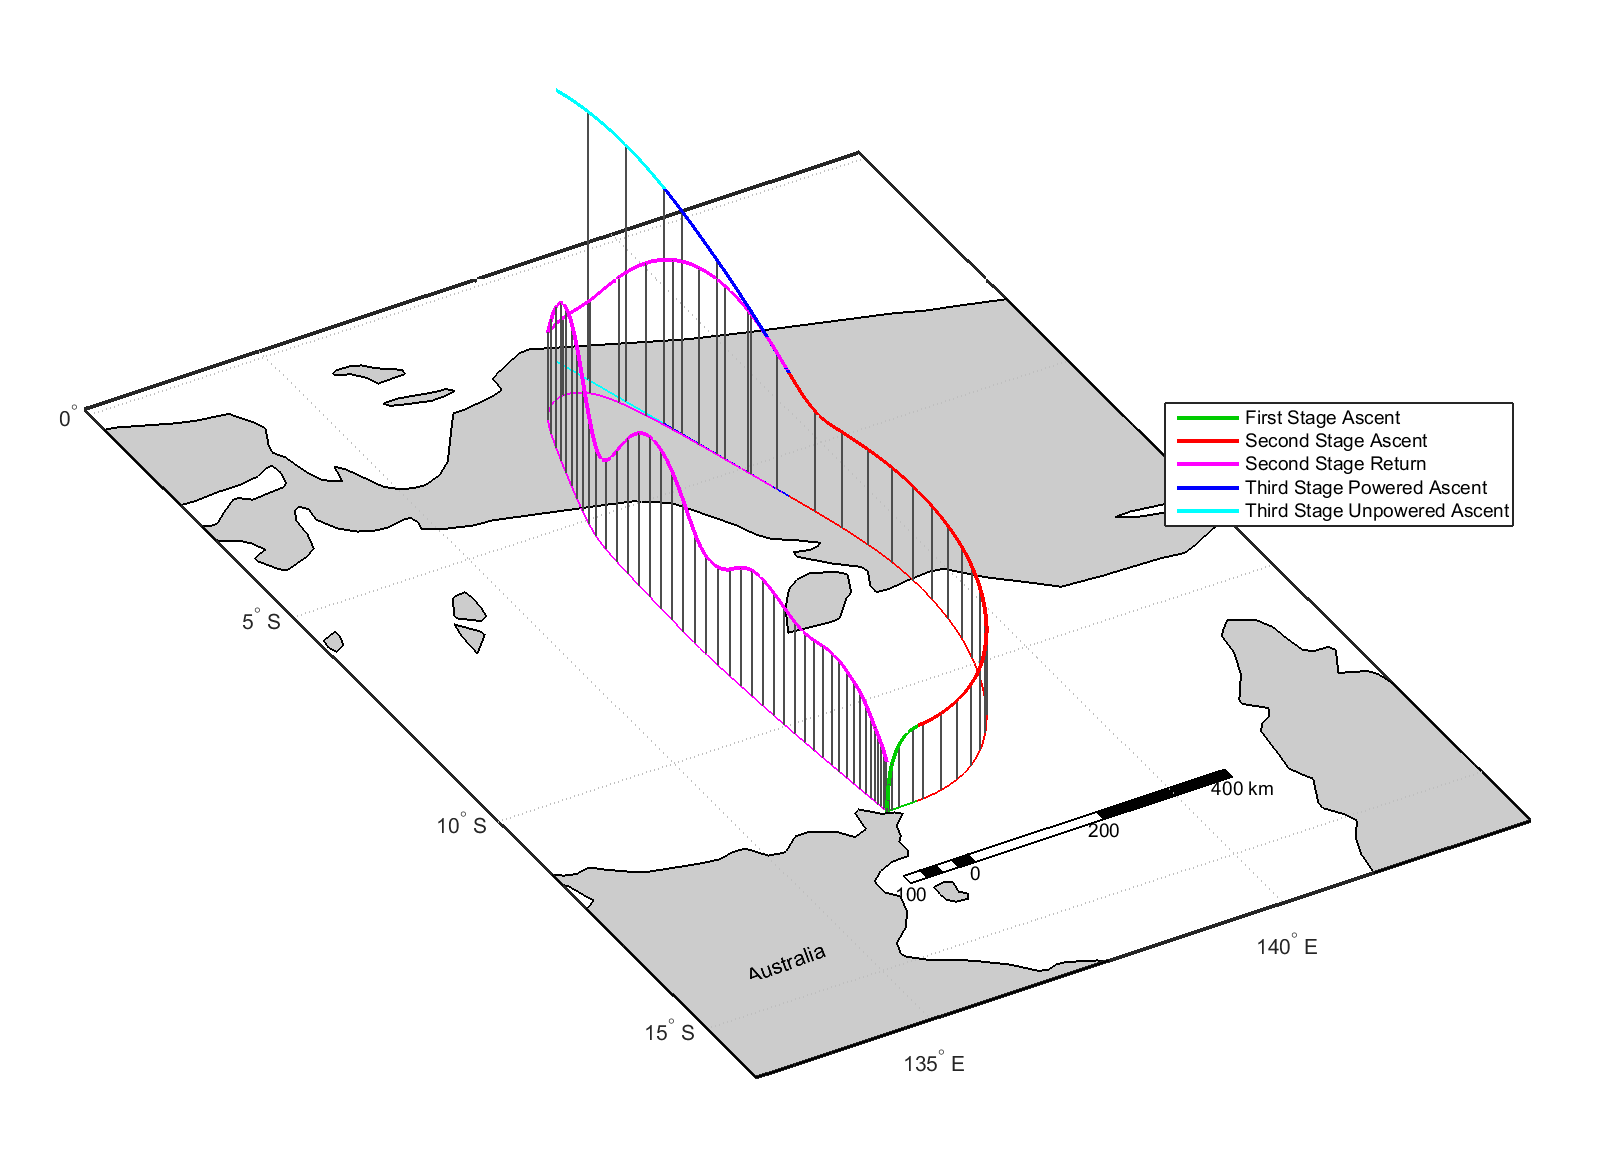
\includegraphics[width=1\linewidth]{../LODESTAR_FINAL/Results/mode11/GroundTrackStandard}
	\caption{}
	\label{fig:GroundTrackStandard}
\end{figure}
The maximum payload-to-orbit is reduced by -10.0\% compared to the optimised trajectory result without fly-back. The benefits of flying back the SPARTAN to its initial launch site, compared to the alternative of transporting the SPARTAN back to the launch site from a remote landing, are likely to far outweigh this associated reduction in payload. 



\section{Ascent Trajectory}

 The initial launch for a maximum payload-to-orbit trajectory with SPARTAN fly-back is to the east.
 The first stage trajectory, shown in Figure \ref{fig:FirstStageStandard}, is very similar to that of the first stage launching the SPARTAN with no return flight, detailed in Section \ref{sec:optimisednoreturn}, with the exception of a small adjustment manoeuvre. 
 After pitchover, the first stage gradually reduces the angle of attack to a minimum of -0.47$^\circ$ at 30.9s flight time, in order to make small adjustments to the pitch profile while the velocity is low. After this, the angle of attack returns to 0$^\circ$ at 42.9s flight time, and is maintained for 16.4s.
 The angle of attack is then reduced, to a minimum of -3.58$^\circ$ in order to adjust the altitude and trajectory angle, before increasing back to 0$^\circ$ at first stage-SPARTAN separation. 
 The SPARTAN is released in an easterly direction, at a heading angle of -12.4$^\circ$, an altitude of \firstsecondSeparationAltStandard km, and a trajectory angle of \firstsecondSeparationgammaStandard $^\circ$. 
 This altitude of first stage-SPARTAN separation is 3.02km (+12.5\%) higher than the first stage-SPARTAN release with no fly-back, and the trajectory angle is 2.5$^\circ$ (80.6\%) higher. 
 This higher release point increases the exergy efficiency of the first stage rocket by 0.426\%$\eta$ (5.2\%), and allows the first stage to achieve a higher velocity at separation (an increase of 64m/s, 4.3\%). 
 
 The higher altitude, larger trajectory angle, and increased velocity at the first stage-SPARTAN separation point causes a large altitude raising manoeuvre at the beginning of the SPARTAN's acceleration. This altitude raising manoeuvre takes the SPARTAN to a height of 29.59km at 31.44s, and decreases the dynamic pressure of the SPARTAN to 29.1kPa, allowing time for the bank angle of the SPARTAN to be increased. 
 The bank angle is initially increased at the maximum change rate to 44.2$^\circ$ after the first stage-SPARTAN separation, which aids the SPARTAN in decreasing its altitude. As the dynamic pressure of the SPARTAN approaches its maximum, the bank angle stops increasing and the angle of attack is increased to 3.24$^\circ$, to provide more lift, slowing the descent of the SPARTAN. 
 The bank angle then begins to increase once more, and as the SPARTAN reaches close to its maximum dynamic pressure at 109.8s, the angle of attack is reduced, and the bank angle reaches 56.8$^\circ$. 

\begin{figure}[ht!]
\centering
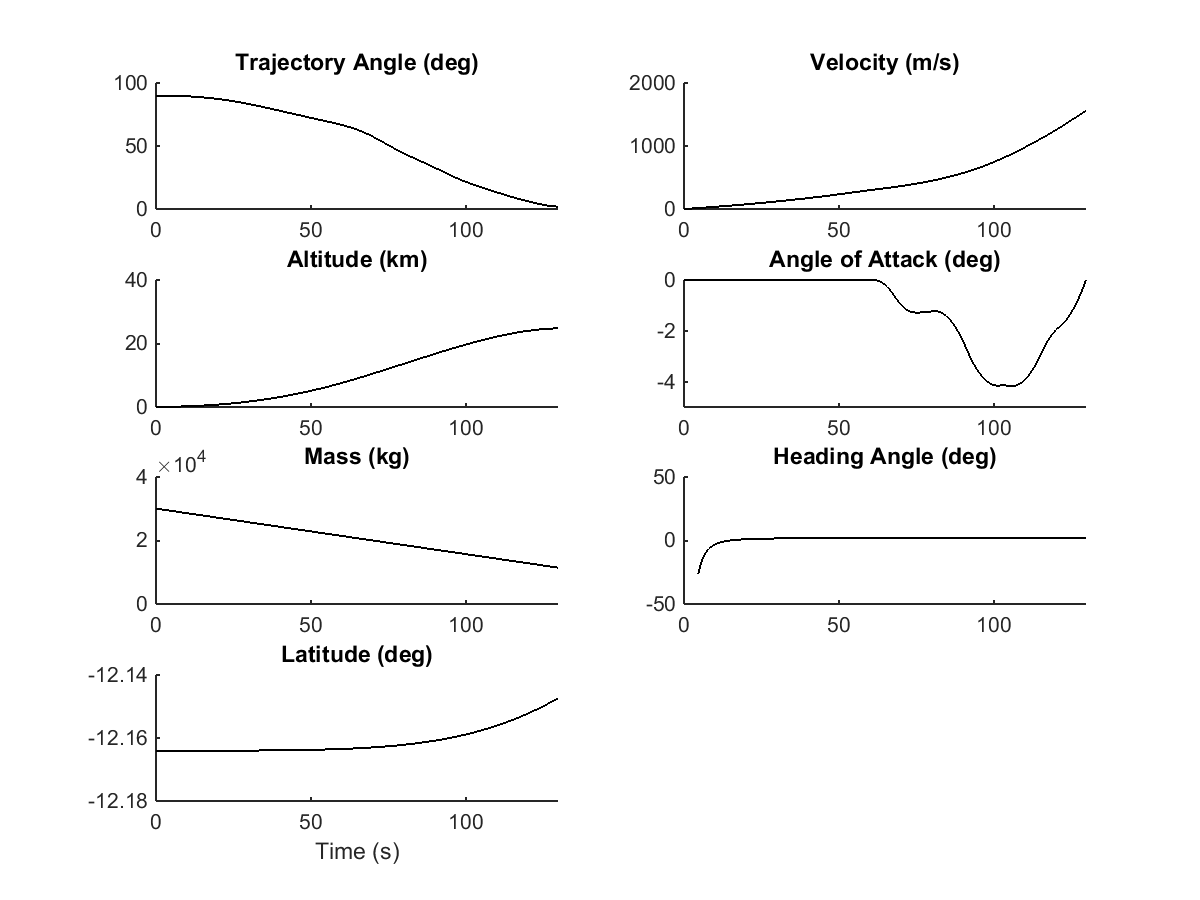
\includegraphics[width=0.7\linewidth]{../LODESTAR_FINAL/Results/mode11/FirstStageStandard}
\caption{}
\label{fig:FirstStageStandard}
\end{figure}
 
\begin{figure}[ht!]
\centering
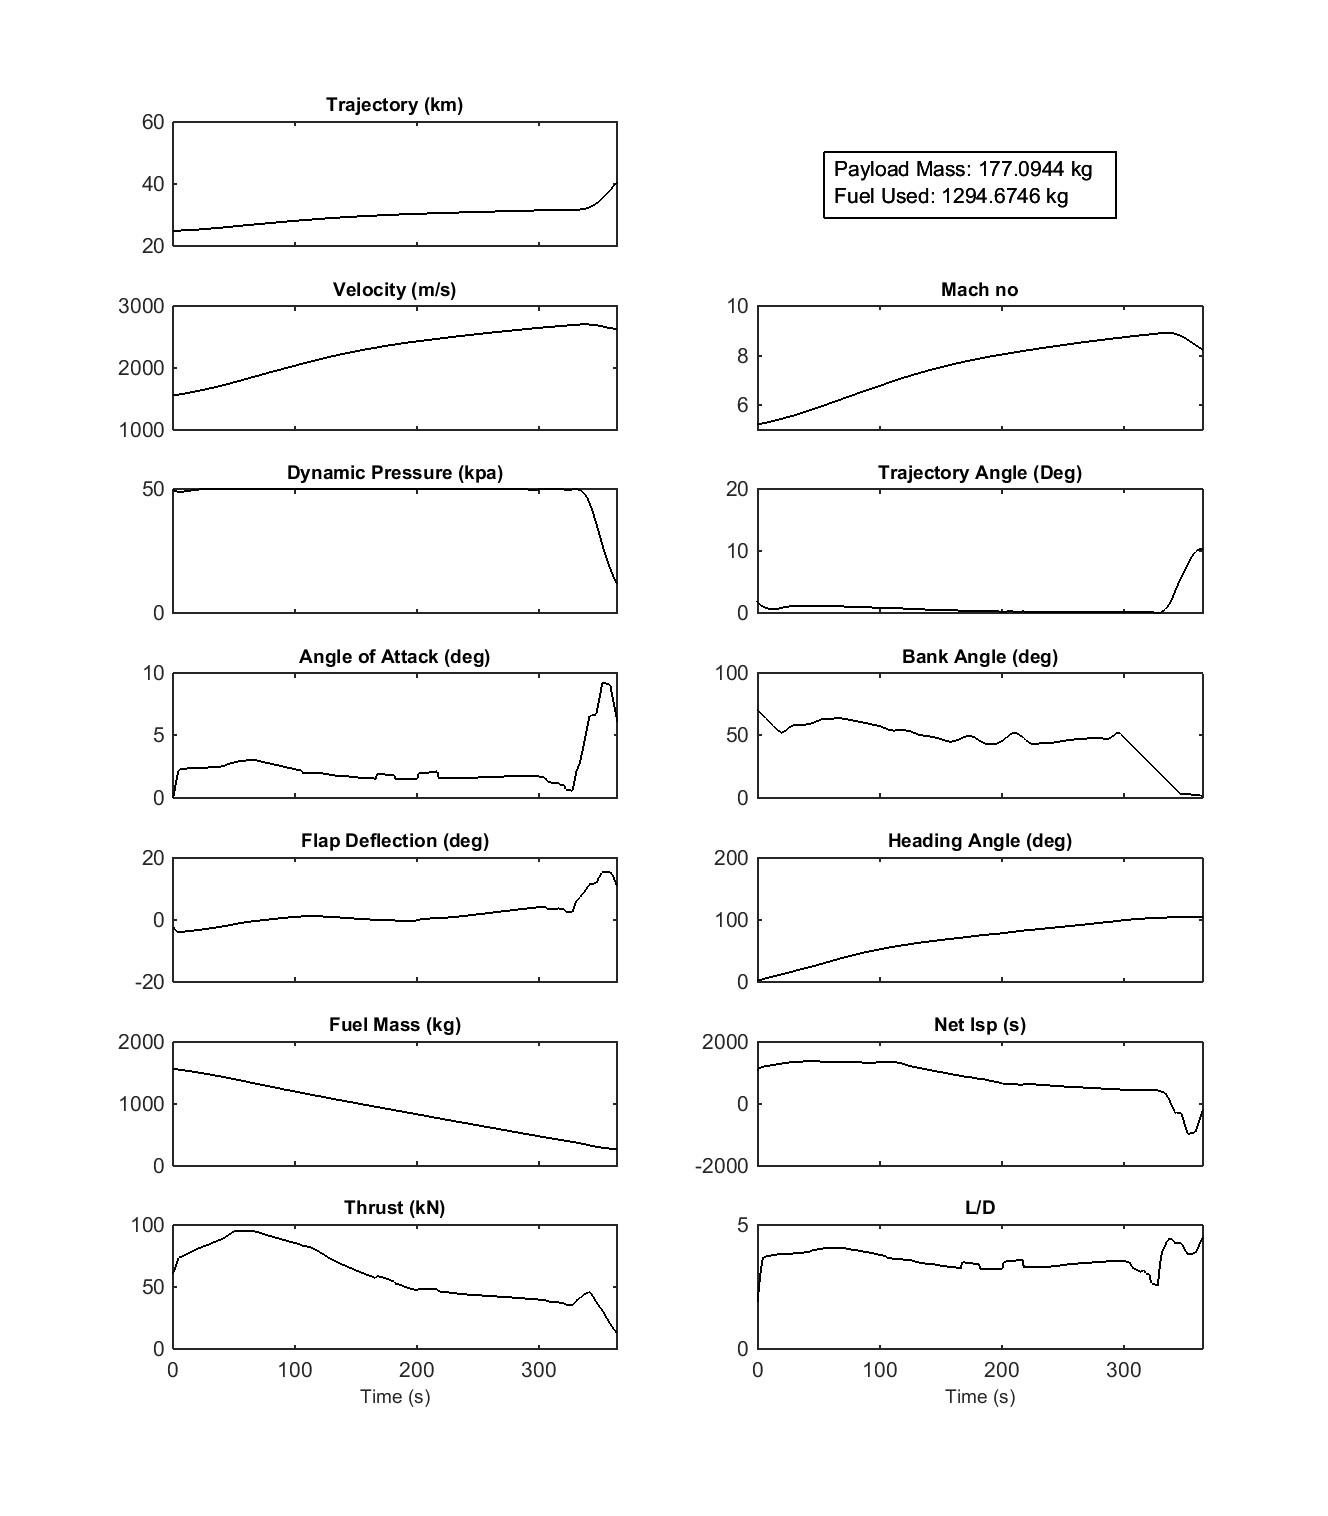
\includegraphics[width=1\linewidth]{../LODESTAR_FINAL/Results/mode11/SecondStageStandard}
\caption{}
\label{fig:SecondStageStandard}
\end{figure}
\begin{figure}[ht!]
\centering
\includegraphics[width=0.9\linewidth]{../LODESTAR_FINAL/Results/mode11/NetIspStandard}
\caption{}
\label{fig:NetIspStandard}
\end{figure}
During the ascent, the bank angle of the SPARTAN is maintained between 50.4$^\circ$ and 58.6$^\circ$, exhibiting higher bank angles towards the latter part of the ascent. 
The angle of attack of the SPARTAN is significantly higher during the trajectory with fly-back inclusion, compared to maximum payload-to-orbit trajectory with no fly-back, detailed in Section \ref{sec:optimisednoreturn}. 

 The higher angles of attack flown by the SPARTAN during the maximum payload-to-orbit trajectory with fly-back results in the SPARTAN flying at close to maximum dynamic pressure for most of the duration of its trajectory, without the altitude raising manoeuvre observed in Section \ref{sec:optimisednoreturn}.
 The increase in angle of attack means that the SPARTAN no longer flies within the homogeneous region of the C-REST engines specific impulse, instead the flight conditions are close to a region where an increase in angle of attack causes a sharp decrease in specific impulse. 
This indicates that at Mach 7 and 8 the angle of attack, and consequently, the allowable bank angle, of the SPARTAN may be being limited by the performance of the C-REST engines. 
 The SPARTAN stays close to its maximum dynamic pressure until a pull-up is performed at 365.8s flight time. During the pull-up, the bank angle is steadily reduced at its maximum change rate, until close to the release of the third stage rocket, which occurs at 0$^\circ$ bank angle. 

The higher angles of attack flown by the SPARTAN also have the consequence of decreasing the net specific impulse of the SPARTAN during its acceleration, with the maximum specific impulse being decreased by -2.5\%.
The overall exergy efficiency of the SPARTAN is decreased, to \secondExergyEffStandard\%$\eta$, a decrease of -1.448\%$\eta$ (-12.2\%). This exergy efficiency decrease is due partially to the decrease in the specific impulse of the scramjet engines, but more significantly is attributed to the fuel necessary for the return flight resulting in less fuel being used during the ascent of the SPARTAN, and thus less 'useful' work being attained from the total fuel mass.
A total fuel mass of \returnFuelStandard kg is used during the SPARTAN's acceleration. This reduction in fuel mass used, along with the reduction in net specific impulse due to the higher angle of attack values, reduces the velocity at SPARTAN-third stage separation by -106m/s (-3.9\%) compared to the maximum payload-to-orbit case with no SPARTAN fly-back. The SPARTAN pulls up to \secondthirdSeparationAltStandard km altitude and \secondthirdSeparationgammaStandard $^\circ$ before SPARTAN-third stage separation, a difference of only -0.8km (-1.9\%) and +0.2$^\circ$ (+1.8\%) compared to the maximum payload-to-orbit trajectory without fly-back. 

The exergy efficiency of the third stage is increased by +0.465\%$\eta$ (+2.3\%) when compared to the maximum payload-to-orbit trajectory with no SPARTAN fly-back. This indicates that there is the efficiency trade-off between the SPARTAN and the third stage favours the third stage rocket more when the fly-back of the SPARTAN is included. This supports the trends observed in Chapter \ref{chapter:Ascent}, that as the overall 'useful' energy availability of the SPARTAN is decreased, the efficiency trade-off shifts in favour of the third stage rocket.  


\begin{figure}[ht!]
\centering
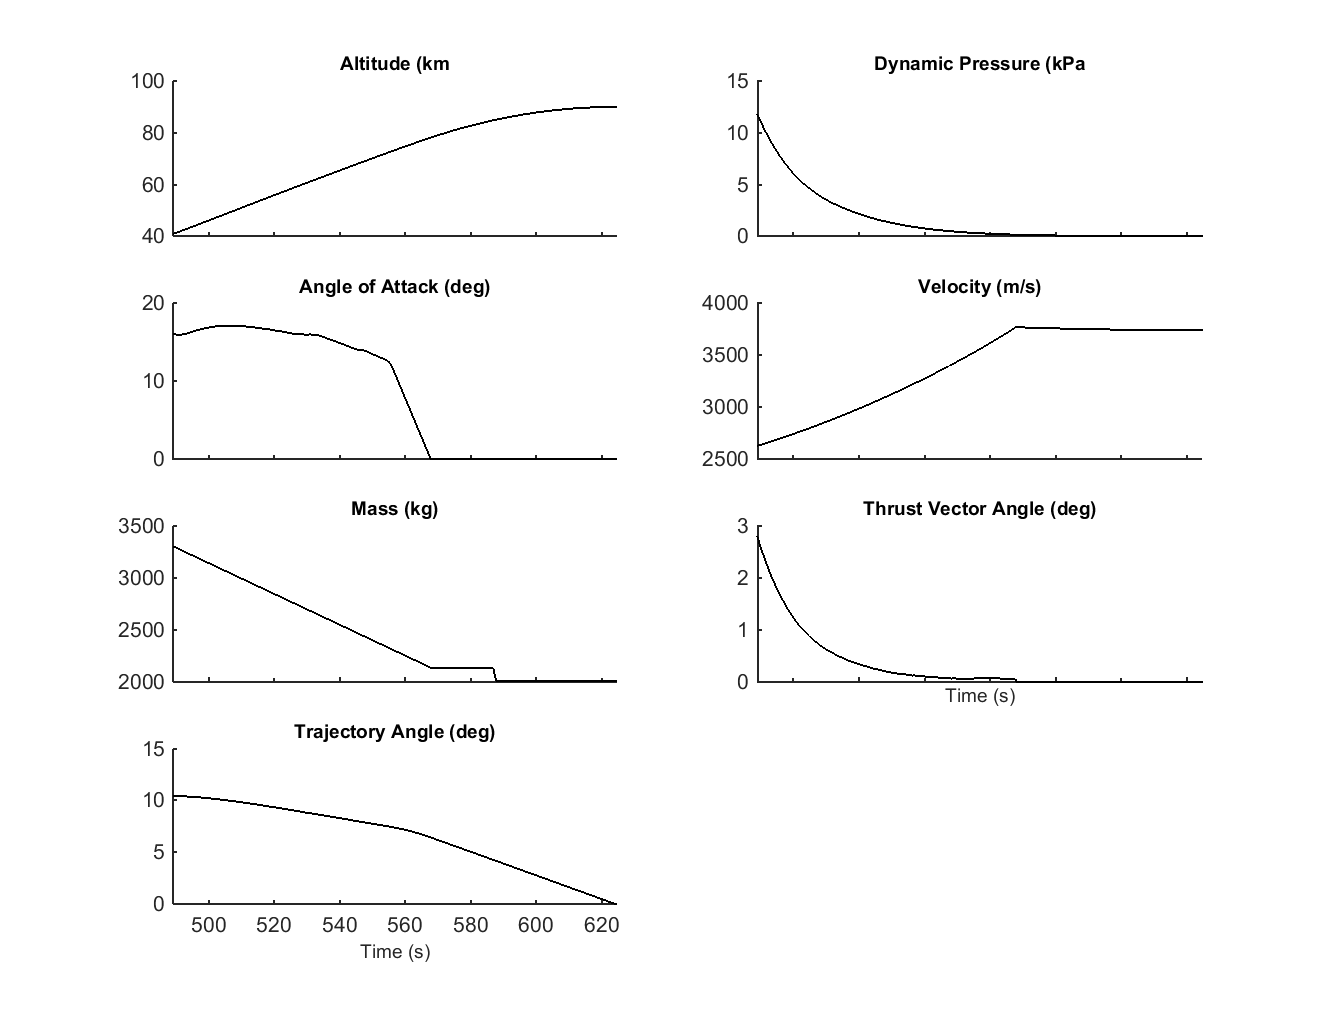
\includegraphics[width=1\linewidth]{../LODESTAR_FINAL/Results/mode11/ThirdStageStandard}
\caption{}
\label{fig:ThirdStageStandard}
\end{figure}


\section{Fly-Back Trajectory}

\begin{figure}[ht!]
	\centering
	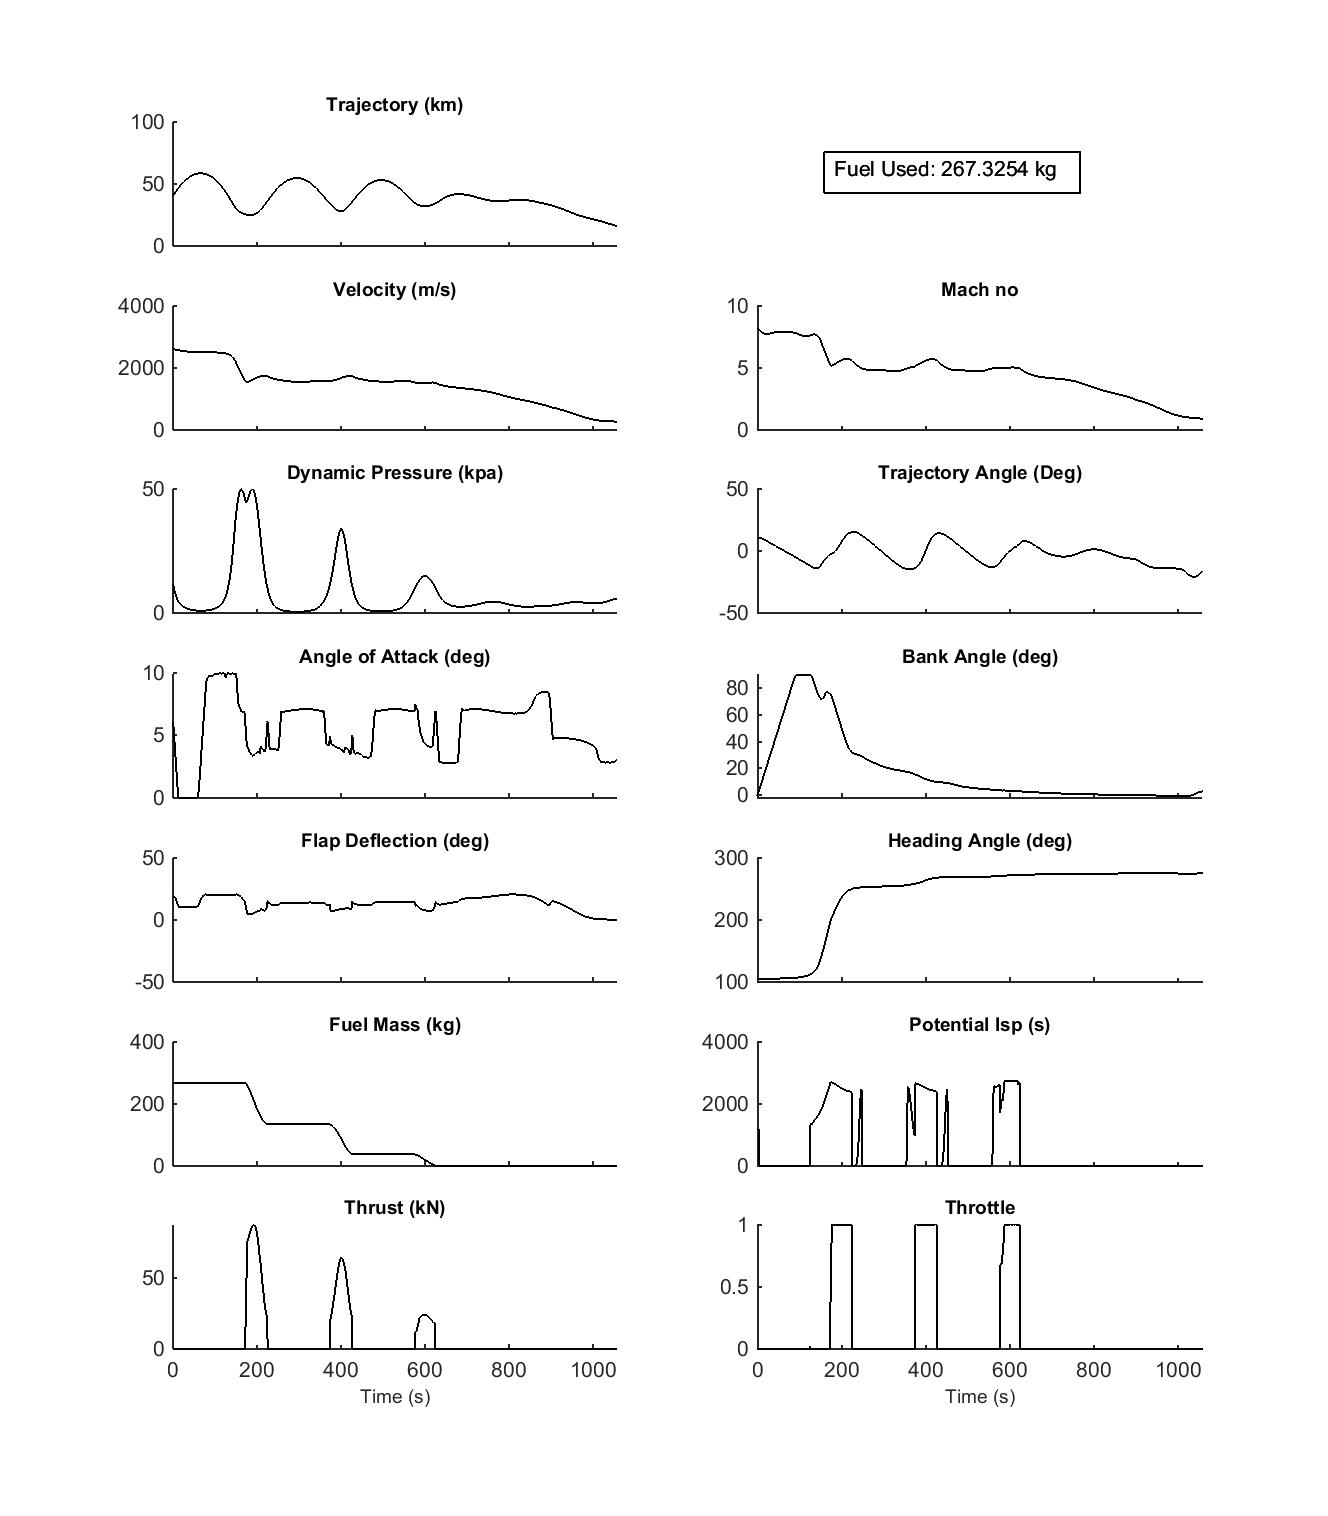
\includegraphics[width=1\linewidth]{../LODESTAR_FINAL/Results/mode11/ReturnStandard}
	\caption{}
	\label{fig:ReturnStandard}
\end{figure}

The optimised fly-back trajectory is shown in Figure \ref{fig:ReturnStandard}.
The SPARTAN is shown to be capable of fly-back, using \returnFuelStandard kg of fuel, 17.2\% of the total fuel.
The optimised trajectory has four distinct parts; 1. initial turn, 2. boost phase, 3. hop-glide, and 4. approach. 
 The skips which the SPARTAN exhibits during its return flight are aided by the angle of attack of the SPARTAN, and are consistent with research which has shown that a periodic skipping trajectory increases the downrange distance achievable by hypersonic vehicles both during powered and unpowered flight\cite{Eggers1957,Kanda2007}. 
 
\subsubsection{ Initial Turn}
The SPARTAN separates from the third stage rocket at a bank angle of 0$^\circ$, and then increases its bank angle at close to the maximum change rate until 108.7s return flight time, at which point 81.7$^\circ$ bank angle is reached.
The angle of attack is kept low during this time, to a minimum of 0.2$^\circ$, in order to minimise the size of the initial skip. 
As the SPARTAN reaches the zenith of its initial skip, at 66.1s flight time and 60.0km altitude, the angle of attack is rapidly increased, up to a maximum of 8.76$^\circ$. 
 At this point, the altitude of the SPARTAN is decreasing, and the SPARTAN rapidly comes close to hitting the maximum dynamic pressure limit of 50kPa. This increase in angle of attack, along with the aid of a reduction in the bank angle to 67.5$^\circ$, generates additional lift to slow the descent of the SPARTAN. 
As the angle of attack of the SPARTAN increases, the high bank angle enables a large heading angle change during the initial phase of the trajectory, particularly at the first trough between the first and second skips. The heading angle increases from 104.8$^\circ$ at the beginning of fly-back, to 221.7$^\circ$ midway through the second skip. This large heading angle change minimises the total ground distance which the SPARTAN must cover during its return, decreasing the fuel mass necessary for fly-back. 

\subsubsection{ Boost Phase}
At 182.8s flight time, as the bank angle is reducing, the scramjet engines are ignited. The C-REST engines are powered-on at a point of high potential specific impulse, at a low Mach number, and initially burn for 22s. The altitude of the SPARTAN is raised during the initial burn, ensuring that the Mach number is kept low for maximum efficiency. The maximum altitude during the burn is limited by the lower dynamic pressure limit of the C-REST engines of 20kPa. 
At 204.8s flight time the initial burn ends, the angle of attack of the SPARTAN is decreased to 3.2$^\circ$, and the SPARTAN executes its second skip. As soon as the dynamic pressure is high enough for C-REST engine operation at 339.9s return flight time, the scramjet engines are once again ignited.
During the second burn, the angle of attack of the SPARTAN is increased, to modify the temperature and Mach number at the inlet of the C-REST engines so that the maximum specific impulse is obtained from the C-REST engines during the burn. 
The angle of attack varies between 4.2$^\circ$ to 3.3$^\circ$ during the second burn. 
This skip raises the altitude of the SPARTAN to 54.6km, before it decreases once again. 
The third and last burn is initiated at 536.7s and lasts until 579.0s, when the remaining fuel has been depleted. Before the third burn, the angle of attack is decreased, so that it varies between 4.5$^\circ$ and 3.7$^\circ$ during the burn. These angle fo attack values are similar to those observed during the second burn, indicating that these angle of attack values obtain a high specific impulse from the C-REST engines, this can be observed in Figure \ref{fig:returnIspStandard}. 


\subsubsection{ Approach}

During the unpowered trajectory, after the third burn phase, the angle of attack is initially controlled so that the skipping trajectory of the SPARTAN is dampened.
Immediately after the third burn phase, the angle of attack is reduced, to 2.82$^\circ$. This reduction coincides with the ascent portion of the fourth skip, reducing the amount of altitude gained. 
As the zenith of the forth skip is reached, the angle of attack is increased to 7.2$^\circ$, once again counteracting the skipping manoeuvre. 
This high angle of attack is sustained until 748.2s at which point the angle of attack is reduced again significantly, to 2.6$^\circ$, reducing the size of the fifth skip significantly. At 871.2s, the angle of attack is again raised to 5$^\circ$, initiating the sixth and last skip.
It is notable that the sixth skip is initiated in this way, as previously in the unpowered portion of the trajectory the angle of attack is being utilised to damped the skipping motion. This indicates that some degree of skipping is desirable, and that the angle of attack is being controlled to produce optimally sized skips. 

After the final small skip, the angle of attack is adjusted, so that a gradual, controlled descent is initiated. 
After the skip phase, as the vehicle is approaching Mach 1, the angle of attack is reduced gradually to bring the SPARTAN down to 1km altitude, in a controlled manner. At 1227.0s, the bank angle is increased, in order to perform a final adjustment of the heading angle, to bring the SPARTAN to the desired end location. 
The SPARTAN reaches 1km altitude at -26.7$^\circ$ trajectory angle and 120.0m/s velocity. It is assumed that the SPARTAN is able to perform a landing manoeuvre after this point. 








\section{Design Sensitivity Analysis}

It has been shown that the fly-back of the SPARTAN accelerator has a significant effect on the performance of the rocket-scramjet-rocket launch system, and that the maximum payload-to-orbit optimised trajectory changes significantly to compensate for the additional requirement of successfully returning the SPARTAN stage. The sensitivity of the launch system to changes in the vehicle design may be significantly affected by the fly-back trajectory, and as such, a sensitivity study is conducted with the fly-back of the SPARTAN included. As in Section \ref{sec:sensitivityNoReturn} this sensitivity study varies the following:
\begin{itemize}
	\item Dynamic Pressure
	\item Specific Impulse
	\item SPARTAN Drag
	\item SPARTAN Mass
	\item SPARTAN Fuel Mass
	\item Third Stage Mass
	\item Third Stage Thrust
\end{itemize}
As in Section \ref{sec:sensitivityNoReturn}, the effect of third stage drag is negligible. For this reason, variation in the third stage drag is omitted from this study. 



In addition to investigating the trends in the performance of the launch system, this sensitivity study serves to verify the ability of LODESTAR to generate optimal trajectories with varied vehicle designs, as well as investigating the robustness of the optimised solution.
The launch system is able to successfully place a small satellite in orbit for every varied performance condition which has been tested, while returning the SPARTAN to its initial launch location for landing. 
Every maximum payload-to-orbit optimised trajectory exhibits considerable banking during the SPARTAN's ascent trajectory, as well as a pull-up of the SPARTAN before third stage release. 
In every case the optimised return flight path exhibits an initial turn, boost and approach phase, with multiple skipping manoeuvres. 
However, two aspects of the optimised trajectories vary between cases, exhibiting no clear trend across the sensitivity studies which have been performed; the first stage-SPARTAN release conditions, and the size of the second skip of the return phase. 

\textcolor{red}{I need to make sure this is correct after all solutions are run}

\textcolor{red}{i may be making too big of a deal about this, note similar work done}
The first stage-SPARTAN separation angle and altitude shows no clear trend in any of the sensitivity studies performed, in contrast to the sensitivity study with no fly-back, detailed in Section XX, in which the mass and drag parameters change the first stage release significantly. All of the optimised trajectory solutions show a distinct initial altitude raising manoeuvre, however, their size is inconsistent across optimised trajectory solutions, indicating that this manoeuvre is no longer solely a product of an efficiency trade-off between the first stage pitching and SPARTAN engine efficiency. When fly-back is included and the SPARTAN is banking, this altitude raising manoeuvre allows large bank angles, changing the heading angle of the SPARTAN rapidly, while maintaining low angles of attack for efficiency. 
In the maximum payload-to-orbit optimised trajectories calculated during the sensitivity analysis, it is observed that the trajectory angle at first-second stage release varies significantly between the optimised trajectories, in often unpredictable ways. When the SPARTAN is released at a high trajectory angle, there is a significant amount of time allowed for the bank angle to increase, and the high bank angle is utilised during the descent of the SPARTAN onto the maximum dynamic pressure path, where the trajectory angle is negative and the heading angle changes more rapidly. 
When the trajectory angle at release of the SPARTAN is lower, the first stage is generally XX \textcolor{red}{look at exergy analysis}. A lower release angle results in the SPARTAN banking more, and flying a slightly less efficient trajectory. However, a lower release angle also results in the SPARTAN using its fuel more rapidly, and covering less ground, which results in the fly-back requiring less fuel. 
The trade-off between first stage efficiency and the initial operational efficiency of the SPARTAN appears to be close, and 
for each particular trajectory optimisation one or the other is favoured. 


It is also observed that there are two distinct return trajectory shapes for the return trajectory of the SPARTAN. The more common return trajectory shape has been shown in the preceding section, and consists of three or more large skips to begin the return trajectory. The second trajectory shape exhibits a small second skip, with the first two burns very closely spaced, or combined into one longer burn. During the first two burns, a high bank angle is maintained  when compared to the large skip trajectory shape, however, after the first two burns are completed, the bank angle is reduced more rapidly. 
An example of the second type of return trajectory is shown in Figure XX(appendix). 
During simulations, it was observed that on occasion, the optimal return trajectory type would change as the initial guess or problem setup was altered, with no significant change in the fuel mass used during the return, or the payload-to-orbit capabilities of the launch system. This variability suggests that there is minimal difference between the two shapes of return trajectory. 





\subsection{Case 12: Dynamic Pressure Variation with Fly-Back Inclusion}

\textcolor{red}{need to redo these tables for new exergy efficiency calculation, and change discussion a little}

The maximum dynamic pressure of the SPARTAN has a slightly increased effect on the variation in the maximum payload-to-orbit, by percentage, when the fly-back of the SPARTAN is included. 
Table \ref{tab:qvarreturn} shows a summary of the key parameters of each optimised trajectory, and trajectory comparison plots are shown in Appendix XX. The variation in each trajectory parameter per \% of the dynamic pressure is shown, if there is a clear trend. The payload-to-orbit of the launch system improves by +9.4kg (+5.51\%) at 60kPa, and decreases by -7.7kg (-4.52\%) at 40kPa.
the overall exergy efficiency of the system increases as the maximum dynamic pressure increases, by +0.06\% at 60kPa, and decreases as the maximum dynamic pressure decreases, by -0.062\% at 40kpa. 

The trends in the exergy efficiencies of each stage are obfuscated by addition of the manoeuvrability of the SPARTAN as a parameter in the trajectory optimisation. The trade-offs between the efficiencies of the stages must also include the manoeuvrability of the SPARTAN which dictates the fuel used during the return flight. This additional factor produces complicated energy trade-offs, which do not produce clear trends with maximum dynamic pressure variation. The 45kPa maximum dynamic pressure simulation in particular shows lower exergy efficiencies for every stage during the ascent when compared to the 40kpa maximum dynamic pressure trajectory, while also producing a higher total exergy efficiency. however, the 45kPa simulation trades off the performance of the stages during ascent to achieve greater manoeuvrability at the beginning of its trajectory. The first stage-SPARTAN separation occurs at a lower altitude and trajectory angle compared to the other simulations, allowing the acceleration to be achieved more quickly at the start of the trajectory, and enabling the SPARTAN to manoeuvre effectively. 
 As a consequence, the 45kPa simulation uses only 257.0kg of fuel during the fly-back, less than the 292.4kg of fuel used by the fly-back of the 40kpa trajectory, as well as the the 268.0kg of fuel used by the fly-back of the 50kPa maximum dynamic pressure trajectory, against the general trend of the return fuel usage. This lower fuel usage during the return flight allows for more fuel usage during the ascent, so that overall, more energy is used towards 'useful' work during the SPARTAN's acceleration. 

Excluding the 45kpa trajectory, it can be observed that generally, increasing the maximum dynamic pressure improves the manoeuvring capabilities of the SPARTAN and increases the acceleration rate during ascent, which leads to a smaller flight time, and less ground coverage, reducing the amount of fuel necessary for fly-back. 
The exergy efficiency of the first stage is generally increased as the maximum dynamic pressure is increased, and the altitude at first stage-SPARTAN release is raised, again with the exception of the 45kpa case. 
The exergy efficiency of the SPARTAN is relatively consistent across the simulations, particularly when compared to the variance observed in the dynamic pressure sensitivity study with no fly-back, in Section \ref{sec:qvariation}.
This is due to the higher maximum dynamic pressure simulations using more fuel during the acceleration of the SPARTAN, and accelerating more over the trajectory (the velocity at SPARTAN-third stage separation increases by +51m/s, 2.0\%, at 60kpa maximum dynamic pressure, and decreases by -28m/s, 1.1\%, at 40kPa), resulting in the specific impulse of the scramjet engines being lower at the end of the acceleration. Overall, the SPARTAN is utilising more fuel mass at similar efficiencies, so that more overall 'useful' work is being gained. 



\begin{table}[ht]
\centering
\begin{tabular}{l c c c c c c} 
	\hline \textbf{Trajectory Condition}
	&q40
	&q45
	&q
	&q55
	&q60
	& $\Delta/\Delta$/\%
	\\
	\hline \textbf{Payload to Orbit (kg)}
	& \textbf{\PayloadToOrbitqForty}
	& \textbf{\PayloadToOrbitqFortyFive}
	& \textbf{\PayloadToOrbitqStandard}
	& \textbf{\PayloadToOrbitqFiftyFive}
	& \textbf{\PayloadToOrbitqSixty}
	&\textbf{0.4}
	\\
	\textbf{Payload Variation (\%)}
	& \PayloadVarqForty
	& \PayloadVarqFortyFive
	& \PayloadVarqStandard
	& \PayloadVarqFiftyFive
	& \PayloadVarqSixty
	&0.25
	\\
	\textbf{Total $\eta_{exergy}$ (\%)}
	& \textbf{\totalExergyEffqForty}
	& \textbf{\totalExergyEffqFortyFive}
	& \textbf{\totalExergyEffqStandard}
	& \textbf{\totalExergyEffqFiftyFive}
	& \textbf{\totalExergyEffqSixty}
	& \textbf{3e-05}
	\\
	\hline 
	\textbf{1$^{st}$ Stage $\eta_{exergy}$ (\%)}
	& \textbf{\firstExergyEffqForty}
	& \textbf{\firstExergyEffqFortyFive}
	& \textbf{\firstExergyEffqStandard}
	& \textbf{\firstExergyEffqFiftyFive}
	& \textbf{\firstExergyEffqSixty}
	& -
	\\
	\textbf{Separation Alt, 1$\rightarrow$2 (km)}
	& \firstsecondSeparationAltqForty
	& \firstsecondSeparationAltqFortyFive
	& \firstsecondSeparationAltqStandard
	& \firstsecondSeparationAltqFiftyFive
	& \firstsecondSeparationAltqSixty
	& -
	\\
	\textbf{Separation v, 1$\rightarrow$2 (m/s)}
	& \firstsecondSeparationvqForty
	& \firstsecondSeparationvqFortyFive
	& \firstsecondSeparationvqStandard
	& \firstsecondSeparationvqFiftyFive
	& \firstsecondSeparationvqSixty
	& -
	\\
	\textbf{Separation $\gamma$, 1$\rightarrow$2 (m/s)}
	& \firstsecondSeparationgammaqForty
	& \firstsecondSeparationgammaqFortyFive
	& \firstsecondSeparationgammaqStandard
	& \firstsecondSeparationgammaqFiftyFive
	& \firstsecondSeparationgammaqSixty
	& -
	\\
	\hline 
	\textbf{2$^{nd}$ Stage $\eta_{exergy}$ (\%)}
	& \textbf{\secondExergyEffqForty}
	& \textbf{\secondExergyEffqFortyFive}
	& \textbf{\secondExergyEffqStandard}
	& \textbf{\secondExergyEffqFiftyFive}
	& \textbf{\secondExergyEffqSixty}
	& -
	\\
	\textbf{Separation Alt, 2$\rightarrow$3 (km)}
	& \secondthirdSeparationAltqForty
	& \secondthirdSeparationAltqFortyFive
	& \secondthirdSeparationAltqStandard
	& \secondthirdSeparationAltqFiftyFive
	& \secondthirdSeparationAltqSixty
	&-0.02
	\\
	\textbf{Separation $v$, 2$\rightarrow$3 (m/s)}
	& \secondthirdSeparationvqForty
	& \secondthirdSeparationvqFortyFive
	& \secondthirdSeparationvqStandard
	& \secondthirdSeparationvqFiftyFive
	& \secondthirdSeparationvqSixty
	&1.99
	\\
	\textbf{Separation $\gamma$, 2$\rightarrow$3 (deg)}
	& \secondthirdSeparationgammaqForty
	& \secondthirdSeparationgammaqFortyFive
	& \secondthirdSeparationgammaqStandard
	& \secondthirdSeparationgammaqFiftyFive
	& \secondthirdSeparationgammaqSixty
	& -
	\\
	\textbf{Separation $q$, 2$\rightarrow$3(kPa)}
	& \secondthirdSeparationqqForty
	& \secondthirdSeparationqqFortyFive
	& \secondthirdSeparationqqStandard
	& \secondthirdSeparationqqFiftyFive
	& \secondthirdSeparationqqSixty
	&0.04
	\\
	\textbf{2$^{nd}$ Stage L/D, 2$\rightarrow$3}
	& \secondthirdSeparationLDqForty
	& \secondthirdSeparationLDqFortyFive
	& \secondthirdSeparationLDqStandard
	& \secondthirdSeparationLDqFiftyFive
	& \secondthirdSeparationLDqSixty
	&0.02
	\\
	\textbf{2$^{nd}$ Stage Flight Time (s)}
	& \secondFlightTimeqForty
	& \secondFlightTimeqFortyFive
	& \secondFlightTimeqStandard
	& \secondFlightTimeqFiftyFive
	& \secondFlightTimeqSixty
	&-1.58
	\\
	\hline 
	\textbf{3$^{rd}$ Stage $\eta_{exergy}$ (\%)}
	& \textbf{\thirddExergyEffqForty}
	& \textbf{\thirddExergyEffqFortyFive}
	& \textbf{\thirddExergyEffqStandard}
	& \textbf{\thirddExergyEffqFiftyFive}
	& \textbf{\thirddExergyEffqSixty}
	& -
	\\
	\textbf{2$^{nd}$ Stage Return Fuel (kg)}
	& \returnFuelqForty
	& \returnFuelqFortyFive
	& \returnFuelqStandard
	& \returnFuelqFiftyFive
	& \returnFuelqSixty
	& -
	\\
	\textbf{3$^{rd}$ Stage $t$, $q >$ 5kpa (s)}
	& \thirdqOverFiveqForty
	& \thirdqOverFiveqFortyFive
	& \thirdqOverFiveqStandard
	& \thirdqOverFiveqFiftyFive
	& \thirdqOverFiveqSixty
	& -
	\\
	\textbf{3$^{rd}$ Stage max $\alpha$ (deg)}
	& \thirdmaxAoAqForty
	& \thirdmaxAoAqFortyFive
	& \thirdmaxAoAqStandard
	& \thirdmaxAoAqFiftyFive
	& \thirdmaxAoAqSixty
	&0
	\\
	\textbf{3$^{rd}$ Stage Fuel Mass (kg)}
	& \thirdmFuelqForty
	& \thirdmFuelqFortyFive
	& \thirdmFuelqStandard
	& \thirdmFuelqFiftyFive
	& \thirdmFuelqSixty
	&-0.42
	\\
	\hline 
\end{tabular} 
\caption{}
\label{tab:qvarreturn}
\end{table}


\subsection{Case 13: C-REST Specific Impulse with Fly-Back Inclusion}

The specific impulse of the SPARTAN is varied by $\pm10\%$ in order to assess the sensitivity of the optimised trajectory to the performance of the scramjet engines.  
Similarly to the specific impulse sensitivity study with no fly-back conducted in Section XX, the first stage trajectory is not significantly altered as the specific impulse of the SPARTAN is varied, and consequently the first stage-SPARTAN separation conditions, as well as the exergy efficiency of the first stage, exhibit no clear trends. Following separation, the shape of the SPARTAN's acceleration is very similar with specific impulse variation, including the the pull-up location and acceleration flight times. As with the optimised trajectories with no fly-back, increasing the specific impulse of the scramjet engines by 10\% increases the velocity at separation (by +114m/s, +4.4\%) and decreases the trajectory angle (by -0.7$^\circ$, 6.4\%), while decreasing the specific impulse of the scramjet engines by 10\% decreases the velocity at SPARTAN-third stage separation (by -106m/s, 4.1\%), and increases the trajectory angle (by -1.1$^\circ$, -10\%).

, which directly increases the velocity of the third stage at circularisation.

While an increase in the specific impulse of the SPARTAN's scramjet engines is significantly beneficial, the sensitivity of the trajectory to specific impulse is decreased by XX\% compared to the sensitivity study of the optimised trajectory with no fly-back. 
The specific impulse has a significantly smaller effect on the separation velocity when compared to the sensitivity study with no fly-back. Increasing the specific impulse increases the SPARTAN-third stage separation velocity by only XXm/s/\% compared to XXm/s/\% without fly-back.  
This smaller effect is due to the lower second stage acceleration time, which reduces the additional velocity which can be imparted to the third stage rocket due to the increased specific impulse. 






\begin{table}[ht]
	\centering
\begin{tabular}{l c c c c c c} 
	\hline \textbf{Trajectory Condition}
	&Isp90
	&Isp95
	&Isp
	&Isp105
	&Isp110
	& $\Delta/\Delta$/\%
	\\
	\hline \textbf{Payload to Orbit (kg)}
	& \textbf{\PayloadToOrbitIspNinety}
	& \textbf{\PayloadToOrbitIspNinetyFive}
	& \textbf{\PayloadToOrbitIspStandard}
	& \textbf{\PayloadToOrbitIspOneHundredFive}
	& \textbf{\PayloadToOrbitIspOneHundredTen}
	&\textbf{1.7}
	\\
	\textbf{Payload Variation (\%)}
	& \PayloadVarIspNinety
	& \PayloadVarIspNinetyFive
	& \PayloadVarIspStandard
	& \PayloadVarIspOneHundredFive
	& \PayloadVarIspOneHundredTen
	&0.98
	\\
	\textbf{Total $\eta_{exergy}$ (\%)}
	& \textbf{\totalExergyEffIspNinety}
	& \textbf{\totalExergyEffIspNinetyFive}
	& \textbf{\totalExergyEffIspStandard}
	& \textbf{\totalExergyEffIspOneHundredFive}
	& \textbf{\totalExergyEffIspOneHundredTen}
	& \textbf{0.00015}
	\\
	\hline 
	\textbf{1$^{st}$ Stage $\eta_{exergy}$ (\%)}
	& \textbf{\firstExergyEffIspNinety}
	& \textbf{\firstExergyEffIspNinetyFive}
	& \textbf{\firstExergyEffIspStandard}
	& \textbf{\firstExergyEffIspOneHundredFive}
	& \textbf{\firstExergyEffIspOneHundredTen}
	& -
	\\
	\textbf{Separation Alt, 1$\rightarrow$2 (km)}
	& \firstsecondSeparationAltIspNinety
	& \firstsecondSeparationAltIspNinetyFive
	& \firstsecondSeparationAltIspStandard
	& \firstsecondSeparationAltIspOneHundredFive
	& \firstsecondSeparationAltIspOneHundredTen
	& -
	\\
	\textbf{Separation v, 1$\rightarrow$2 (m/s)}
	& \firstsecondSeparationvIspNinety
	& \firstsecondSeparationvIspNinetyFive
	& \firstsecondSeparationvIspStandard
	& \firstsecondSeparationvIspOneHundredFive
	& \firstsecondSeparationvIspOneHundredTen
	& -
	\\
	\textbf{Separation $\gamma$, 1$\rightarrow$2 (m/s)}
	& \firstsecondSeparationgammaIspNinety
	& \firstsecondSeparationgammaIspNinetyFive
	& \firstsecondSeparationgammaIspStandard
	& \firstsecondSeparationgammaIspOneHundredFive
	& \firstsecondSeparationgammaIspOneHundredTen
	& -
	\\
	\hline 
	\textbf{2$^{nd}$ Stage $\eta_{exergy}$ (\%)}
	& \textbf{\secondExergyEffIspNinety}
	& \textbf{\secondExergyEffIspNinetyFive}
	& \textbf{\secondExergyEffIspStandard}
	& \textbf{\secondExergyEffIspOneHundredFive}
	& \textbf{\secondExergyEffIspOneHundredTen}
	& \textbf{0.141}
	\\
	\textbf{Separation Alt, 2$\rightarrow$3 (km)}
	& \secondthirdSeparationAltIspNinety
	& \secondthirdSeparationAltIspNinetyFive
	& \secondthirdSeparationAltIspStandard
	& \secondthirdSeparationAltIspOneHundredFive
	& \secondthirdSeparationAltIspOneHundredTen
	& -
	\\
	\textbf{Separation $v$, 2$\rightarrow$3 (m/s)}
	& \secondthirdSeparationvIspNinety
	& \secondthirdSeparationvIspNinetyFive
	& \secondthirdSeparationvIspStandard
	& \secondthirdSeparationvIspOneHundredFive
	& \secondthirdSeparationvIspOneHundredTen
	&11.13
	\\
	\textbf{Separation $\gamma$, 2$\rightarrow$3 (deg)}
	& \secondthirdSeparationgammaIspNinety
	& \secondthirdSeparationgammaIspNinetyFive
	& \secondthirdSeparationgammaIspStandard
	& \secondthirdSeparationgammaIspOneHundredFive
	& \secondthirdSeparationgammaIspOneHundredTen
	&-0.09
	\\
	\textbf{Separation $q$, 2$\rightarrow$3(kPa)}
	& \secondthirdSeparationqIspNinety
	& \secondthirdSeparationqIspNinetyFive
	& \secondthirdSeparationqIspStandard
	& \secondthirdSeparationqIspOneHundredFive
	& \secondthirdSeparationqIspOneHundredTen
	& -
	\\
	\textbf{2$^{nd}$ Stage L/D, 2$\rightarrow$3}
	& \secondthirdSeparationLDIspNinety
	& \secondthirdSeparationLDIspNinetyFive
	& \secondthirdSeparationLDIspStandard
	& \secondthirdSeparationLDIspOneHundredFive
	& \secondthirdSeparationLDIspOneHundredTen
	& -
	\\
	\textbf{2$^{nd}$ Stage Flight Time (s)}
	& \secondFlightTimeIspNinety
	& \secondFlightTimeIspNinetyFive
	& \secondFlightTimeIspStandard
	& \secondFlightTimeIspOneHundredFive
	& \secondFlightTimeIspOneHundredTen
	& -
	\\
	\hline 
	\textbf{3$^{rd}$ Stage $\eta_{exergy}$ (\%)}
	& \textbf{\thirddExergyEffIspNinety}
	& \textbf{\thirddExergyEffIspNinetyFive}
	& \textbf{\thirddExergyEffIspStandard}
	& \textbf{\thirddExergyEffIspOneHundredFive}
	& \textbf{\thirddExergyEffIspOneHundredTen}
	& \textbf{-0.061}
	\\
	\textbf{2$^{nd}$ Stage Return Fuel (kg)}
	& \returnFuelIspNinety
	& \returnFuelIspNinetyFive
	& \returnFuelIspStandard
	& \returnFuelIspOneHundredFive
	& \returnFuelIspOneHundredTen
	& -
	\\
	\textbf{3$^{rd}$ Stage $t$, $q >$ 5kpa (s)}
	& \thirdqOverFiveIspNinety
	& \thirdqOverFiveIspNinetyFive
	& \thirdqOverFiveIspStandard
	& \thirdqOverFiveIspOneHundredFive
	& \thirdqOverFiveIspOneHundredTen
	& -
	\\
	\textbf{3$^{rd}$ Stage max $\alpha$ (deg)}
	& \thirdmaxAoAIspNinety
	& \thirdmaxAoAIspNinetyFive
	& \thirdmaxAoAIspStandard
	& \thirdmaxAoAIspOneHundredFive
	& \thirdmaxAoAIspOneHundredTen
	& -
	\\
	\textbf{3$^{rd}$ Stage Fuel Mass (kg)}
	& \thirdmFuelIspNinety
	& \thirdmFuelIspNinetyFive
	& \thirdmFuelIspStandard
	& \thirdmFuelIspOneHundredFive
	& \thirdmFuelIspOneHundredTen
	&-1.67
	\\
	\hline 
\end{tabular} 

\end{table}

\subsection{Cd}

The coefficient of drag is varied by $\pm$10\% to investigate the effect of variation in SPARTAN design on the performance of the launch system, including the effects on the fly-back of the SPARTAN. 

Increasing the drag coefficient causes the fuel necessary for fly-back to increase by +XXkg (+XX\%). Conversely, decreasing the drag coefficient by 10\% causes the fuel necessary for  fly-back to decrease by -XXkg (-XX\%). 
When the drag is increased (ie. L/D is decreased), the velocity decreases more rapidly during the return flight, and results in the initial burn beginning sooner as Cd is increased. 
As the Cd is increased, the size of the second skip is generally decreased, resulting in a shorter gap between the first and second burns. At 110\% drag, there is only one long initial burn, and two total burns. 



As in the drag sensitivity study with no return, the SPARTAN-third stage separation angle shows a general increase as drag in increased. However, in contrast to the drag variation study with no fly-back, increasing the drag of the SPARTAN shows a clear trend in decreasing the altitude of SPARTAN-third stage separation. 
As well as this, the L/D at SPARTAN-third stage separation shows the opposite trend to the sensitivity study with no return, decreasing rather than increasing as drag is increased. This is due to the angle of attack of the SPARTAN being reduced at separation when return is present, resulting in a more efficient L/D, and being reduced more as the drag is decreased. 
The release altitude and angle of attack serve to initiate the first skip of the return trajectory in a consistent manner, so that the shape of the initial skip is very similar with drag variation. In all cases the angle of attack is reduced to 0$^\circ$ immediately during return to lessen the size of the initial skip, and is then raised to close to the maximum of 10$^\circ$ to prevent the dynamic pressure limit being exceeded. This consistency indicates that it is the control and structural limitations of the SPARTAN which are driving the conditions at SPARTAN-third stage release. 


-the effect of Cd is reduced compared to the no fly-back case

-some of the negative effects of Cd are offset by the tighter trajectory being flown, and the lower ground distance covered


\begin{table}[ht]
	\centering
\begin{tabular}{l c c c c c c} 
	\hline \textbf{Trajectory Condition}
	&Cd90
	&Cd95
	&Cd100
	&Cd105
	&Cd110
	& /\%
	\\
	\hline \textbf{Payload to Orbit (kg)}
	& \PayloadToOrbitCdNinety
	& \PayloadToOrbitCdNinetyFive
	& \PayloadToOrbitCdStandard
	& \PayloadToOrbitCdOneHundredFive
	& \PayloadToOrbitCdOneHundredTen
	&-1.5
	\\
	\textbf{Separation Alt, 1$\rightarrow$2 (km)}
	& \firstsecondSeparationAltCdNinety
	& \firstsecondSeparationAltCdNinetyFive
	& \firstsecondSeparationAltCdStandard
	& \firstsecondSeparationAltCdOneHundredFive
	& \firstsecondSeparationAltCdOneHundredTen
	& -
	\\
	\textbf{Separation v, 1$\rightarrow$2 (m/s)}
	& \firstsecondSeparationvCdNinety
	& \firstsecondSeparationvCdNinetyFive
	& \firstsecondSeparationvCdStandard
	& \firstsecondSeparationvCdOneHundredFive
	& \firstsecondSeparationvCdOneHundredTen
	&-3.66
	\\
	\textbf{Separation $\gamma$, 1$\rightarrow$2 (m/s)}
	& \firstsecondSeparationgammaCdNinety
	& \firstsecondSeparationgammaCdNinetyFive
	& \firstsecondSeparationgammaCdStandard
	& \firstsecondSeparationgammaCdOneHundredFive
	& \firstsecondSeparationgammaCdOneHundredTen
	& -
	\\
	\textbf{1st Stage $\Delta$Exergy (GJ)}
	& \firstdExergyCdNinety
	& \firstdExergyCdNinetyFive
	& \firstdExergyCdStandard
	& \firstdExergyCdOneHundredFive
	& \firstdExergyCdOneHundredTen
	&-0.06
	\\
	\textbf{Separation Alt, 2$\rightarrow$3 (km)}
	& \secondthirdSeparationAltCdNinety
	& \secondthirdSeparationAltCdNinetyFive
	& \secondthirdSeparationAltCdStandard
	& \secondthirdSeparationAltCdOneHundredFive
	& \secondthirdSeparationAltCdOneHundredTen
	&-0.04
	\\
	\textbf{Separation $v$, 2$\rightarrow$3 (m/s)}
	& \secondthirdSeparationvCdNinety
	& \secondthirdSeparationvCdNinetyFive
	& \secondthirdSeparationvCdStandard
	& \secondthirdSeparationvCdOneHundredFive
	& \secondthirdSeparationvCdOneHundredTen
	&-9.5
	\\
	\textbf{Separation $\gamma$, 2$\rightarrow$3 (deg)}
	& \secondthirdSeparationgammaCdNinety
	& \secondthirdSeparationgammaCdNinetyFive
	& \secondthirdSeparationgammaCdStandard
	& \secondthirdSeparationgammaCdOneHundredFive
	& \secondthirdSeparationgammaCdOneHundredTen
	& -
	\\
	\textbf{Separation $q$, 2$\rightarrow$3(kPa)}
	& \secondthirdSeparationqCdNinety
	& \secondthirdSeparationqCdNinetyFive
	& \secondthirdSeparationqCdStandard
	& \secondthirdSeparationqCdOneHundredFive
	& \secondthirdSeparationqCdOneHundredTen
	& -
	\\
	\textbf{2$^{nd}$ Stage L/D, 2$\rightarrow$3}
	& \secondthirdSeparationLDCdNinety
	& \secondthirdSeparationLDCdNinetyFive
	& \secondthirdSeparationLDCdStandard
	& \secondthirdSeparationLDCdOneHundredFive
	& \secondthirdSeparationLDCdOneHundredTen
	&-0.05
	\\
	\textbf{2$^{nd}$ Stage Flight Time (s)}
	& \secondFlightTimeCdNinety
	& \secondFlightTimeCdNinetyFive
	& \secondFlightTimeCdStandard
	& \secondFlightTimeCdOneHundredFive
	& \secondFlightTimeCdOneHundredTen
	& -
	\\
	\textbf{2nd Stage $\Delta$Exergy (GJ)}
	& \seconddExergyCdNinety
	& \seconddExergyCdNinetyFive
	& \seconddExergyCdStandard
	& \seconddExergyCdOneHundredFive
	& \seconddExergyCdOneHundredTen
	&-0.15
	\\
	\textbf{2$^{nd}$ Stage Return Fuel (kg)}
	& \returnFuelCdNinety
	& \returnFuelCdNinetyFive
	& \returnFuelCdStandard
	& \returnFuelCdOneHundredFive
	& \returnFuelCdOneHundredTen
	& -
	\\
	\textbf{2nd Stage Return $\Delta$Exergy (GJ)}
	& \returndExergyCdNinety
	& \returndExergyCdNinetyFive
	& \returndExergyCdStandard
	& \returndExergyCdOneHundredFive
	& \returndExergyCdOneHundredTen
	&0.12
	\\
	\textbf{3$^{rd}$ Stage $t$, $q >$ 5kpa (s)}
	& \thirdqOverFiveCdNinety
	& \thirdqOverFiveCdNinetyFive
	& \thirdqOverFiveCdStandard
	& \thirdqOverFiveCdOneHundredFive
	& \thirdqOverFiveCdOneHundredTen
	& -
	\\
	\textbf{3$^{rd}$ Stage max $\alpha$ (deg)}
	& \thirdmaxAoACdNinety
	& \thirdmaxAoACdNinetyFive
	& \thirdmaxAoACdStandard
	& \thirdmaxAoACdOneHundredFive
	& \thirdmaxAoACdOneHundredTen
	& -
	\\
	\textbf{3$^{rd}$ Stage final v (m/s)}
	& \thirdcircvCdNinety
	& \thirdcircvCdNinetyFive
	& \thirdcircvCdStandard
	& \thirdcircvCdOneHundredFive
	& \thirdcircvCdOneHundredTen
	&-8.51
	\\
	\textbf{3$^{rd}$ Stage final m (kg)}
	& \thirdcircmCdNinety
	& \thirdcircmCdNinetyFive
	& \thirdcircmCdStandard
	& \thirdcircmCdOneHundredFive
	& \thirdcircmCdOneHundredTen
	& -
	\\
	\textbf{3rd Stage $\Delta$Exergy (GJ)}
	& \thirddExergyCdNinety
	& \thirddExergyCdNinetyFive
	& \thirddExergyCdStandard
	& \thirddExergyCdOneHundredFive
	& \thirddExergyCdOneHundredTen
	& -
	\\
	\hline 
\end{tabular} 
\end{table}


\subsection{m SPARTAN}


\begin{table}[ht]
\centering
\begin{tabular}{l c c c c c c} 
	\hline \textbf{Trajectory Condition}
	&m
	&m
	&m
	&m
	&m
	& /\%
	\\
	\hline \textbf{Payload to Orbit (kg)}
	& \PayloadToOrbitmSPARTANNinetyFive
	& \PayloadToOrbitmSPARTANNinetySevenFive
	& \PayloadToOrbitmSPARTANStandard
	& \PayloadToOrbitmSPARTANOneHundredTwoFive
	& \PayloadToOrbitmSPARTANOneHundredFive
	&-1.4
	\\
	\textbf{Separation Alt, 1$\rightarrow$2 (km)}
	& \firstsecondSeparationAltmSPARTANNinetyFive
	& \firstsecondSeparationAltmSPARTANNinetySevenFive
	& \firstsecondSeparationAltmSPARTANStandard
	& \firstsecondSeparationAltmSPARTANOneHundredTwoFive
	& \firstsecondSeparationAltmSPARTANOneHundredFive
	& -
	\\
	\textbf{Separation v, 1$\rightarrow$2 (m/s)}
	& \firstsecondSeparationvmSPARTANNinetyFive
	& \firstsecondSeparationvmSPARTANNinetySevenFive
	& \firstsecondSeparationvmSPARTANStandard
	& \firstsecondSeparationvmSPARTANOneHundredTwoFive
	& \firstsecondSeparationvmSPARTANOneHundredFive
	&-7.84
	\\
	\textbf{Separation $\gamma$, 1$\rightarrow$2 (m/s)}
	& \firstsecondSeparationgammamSPARTANNinetyFive
	& \firstsecondSeparationgammamSPARTANNinetySevenFive
	& \firstsecondSeparationgammamSPARTANStandard
	& \firstsecondSeparationgammamSPARTANOneHundredTwoFive
	& \firstsecondSeparationgammamSPARTANOneHundredFive
	& -
	\\
	\textbf{1st Stage $\Delta$Exergy (GJ)}
	& \firstdExergymSPARTANNinetyFive
	& \firstdExergymSPARTANNinetySevenFive
	& \firstdExergymSPARTANStandard
	& \firstdExergymSPARTANOneHundredTwoFive
	& \firstdExergymSPARTANOneHundredFive
	&-0.09
	\\
	\textbf{Separation Alt, 2$\rightarrow$3 (km)}
	& \secondthirdSeparationAltmSPARTANNinetyFive
	& \secondthirdSeparationAltmSPARTANNinetySevenFive
	& \secondthirdSeparationAltmSPARTANStandard
	& \secondthirdSeparationAltmSPARTANOneHundredTwoFive
	& \secondthirdSeparationAltmSPARTANOneHundredFive
	&-0.06
	\\
	\textbf{Separation $v$, 2$\rightarrow$3 (m/s)}
	& \secondthirdSeparationvmSPARTANNinetyFive
	& \secondthirdSeparationvmSPARTANNinetySevenFive
	& \secondthirdSeparationvmSPARTANStandard
	& \secondthirdSeparationvmSPARTANOneHundredTwoFive
	& \secondthirdSeparationvmSPARTANOneHundredFive
	&-8.52
	\\
	\textbf{Separation $\gamma$, 2$\rightarrow$3 (deg)}
	& \secondthirdSeparationgammamSPARTANNinetyFive
	& \secondthirdSeparationgammamSPARTANNinetySevenFive
	& \secondthirdSeparationgammamSPARTANStandard
	& \secondthirdSeparationgammamSPARTANOneHundredTwoFive
	& \secondthirdSeparationgammamSPARTANOneHundredFive
	& -
	\\
	\textbf{Separation $q$, 2$\rightarrow$3(kPa)}
	& \secondthirdSeparationqmSPARTANNinetyFive
	& \secondthirdSeparationqmSPARTANNinetySevenFive
	& \secondthirdSeparationqmSPARTANStandard
	& \secondthirdSeparationqmSPARTANOneHundredTwoFive
	& \secondthirdSeparationqmSPARTANOneHundredFive
	& -
	\\
	\textbf{2$^{nd}$ Stage L/D, 2$\rightarrow$3}
	& \secondthirdSeparationLDmSPARTANNinetyFive
	& \secondthirdSeparationLDmSPARTANNinetySevenFive
	& \secondthirdSeparationLDmSPARTANStandard
	& \secondthirdSeparationLDmSPARTANOneHundredTwoFive
	& \secondthirdSeparationLDmSPARTANOneHundredFive
	& -
	\\
	\textbf{2$^{nd}$ Stage Flight Time (s)}
	& \secondFlightTimemSPARTANNinetyFive
	& \secondFlightTimemSPARTANNinetySevenFive
	& \secondFlightTimemSPARTANStandard
	& \secondFlightTimemSPARTANOneHundredTwoFive
	& \secondFlightTimemSPARTANOneHundredFive
	& -
	\\
	\textbf{2nd Stage $\Delta$Exergy (GJ)}
	& \seconddExergymSPARTANNinetyFive
	& \seconddExergymSPARTANNinetySevenFive
	& \seconddExergymSPARTANStandard
	& \seconddExergymSPARTANOneHundredTwoFive
	& \seconddExergymSPARTANOneHundredFive
	&0.06
	\\
	\textbf{2$^{nd}$ Stage Return Fuel (kg)}
	& \returnFuelmSPARTANNinetyFive
	& \returnFuelmSPARTANNinetySevenFive
	& \returnFuelmSPARTANStandard
	& \returnFuelmSPARTANOneHundredTwoFive
	& \returnFuelmSPARTANOneHundredFive
	& -
	\\
	\textbf{3$^{rd}$ Stage $t$, $q >$ 5kpa (s)}
	& \thirdqOverFivemSPARTANNinetyFive
	& \thirdqOverFivemSPARTANNinetySevenFive
	& \thirdqOverFivemSPARTANStandard
	& \thirdqOverFivemSPARTANOneHundredTwoFive
	& \thirdqOverFivemSPARTANOneHundredFive
	& -
	\\
	\textbf{3$^{rd}$ Stage max $\alpha$ (deg)}
	& \thirdmaxAoAmSPARTANNinetyFive
	& \thirdmaxAoAmSPARTANNinetySevenFive
	& \thirdmaxAoAmSPARTANStandard
	& \thirdmaxAoAmSPARTANOneHundredTwoFive
	& \thirdmaxAoAmSPARTANOneHundredFive
	& -
	\\
	\textbf{3$^{rd}$ Stage Circularisation v (m/s)}
	& \thirdcircvmSPARTANNinetyFive
	& \thirdcircvmSPARTANNinetySevenFive
	& \thirdcircvmSPARTANStandard
	& \thirdcircvmSPARTANOneHundredTwoFive
	& \thirdcircvmSPARTANOneHundredFive
	& -
	\\
	\textbf{3$^{rd}$ Stage Circularisation m (kg)}
	& \thirdcircmmSPARTANNinetyFive
	& \thirdcircmmSPARTANNinetySevenFive
	& \thirdcircmmSPARTANStandard
	& \thirdcircmmSPARTANOneHundredTwoFive
	& \thirdcircmmSPARTANOneHundredFive
	& -
	\\
	\textbf{3$^{rd}$ Stage $\Delta$Exergy (GJ)}
	& \thirddExergymSPARTANNinetyFive
	& \thirddExergymSPARTANNinetySevenFive
	& \thirddExergymSPARTANStandard
	& \thirddExergymSPARTANOneHundredTwoFive
	& \thirddExergymSPARTANOneHundredFive
	& -
	\\
	\textbf{Total $\Delta$Exergy (GJ)}
	& \totaldExergymSPARTANNinetyFive
	& \totaldExergymSPARTANNinetySevenFive
	& \totaldExergymSPARTANStandard
	& \totaldExergymSPARTANOneHundredTwoFive
	& \totaldExergymSPARTANOneHundredFive
	& -
	\\
	\hline 
\end{tabular} 

\end{table}





The mass of the SPARTAN is varied by $\pm$5\% to investigate the sensitivity of the launch system performance to the structural mass of the second stage with the inclusion of the fly-back of the SPARTAN. 
Varying the structural mass of the SPARTAN yields a change in potential payload-mass to orbit of 1.2kg per \% of structural mass variation. 
The ascent trajectory varies little with variation in the mass of the SPARTAN. The lower velocity of first stage-SPARTAN separation means that when the SPARTAN is heavier, it is flying at lower velocities, which is beneficial for the specific impulse of the C-REST engines. For this reason, the heavier the SPARTAN is, the more acceleration is obtained over the scramjet-powered ascent. 
Increasing the mass of the SPARTAN decreases the velocity at the end of the first stage by XX\%. Increasing the mass also decreases the altitude of first stage-SPARTAN separation by XX\%. 
It was shown previously in Section XX that decreasing the velocity at first stage-SPARTAN separation does not necessarily affect the altitude of separation. The altitude decrease that is observed is likely to be caused by the increased mass of the SPARTAN requiring greater angle of attack to pull out of the initial altitude raising manoeuvre. As the mass of the SPARTAN increases, the angle of attack is raised for XXs longer to pull out of the descent onto a constant dynamic pressure path, and the decrease in altitude partially offsets the need for this manoeuvre. 

The performance of the launch system shows less sensitivity to the mass of the SPARTAN in the presence of fly-back, 1.2kg/\% compared to 1.5kg/\% without SPARTAN fly-back. 
The sensitivity of the SPARTAN-third stage separation velocity is correspondingly lower, -7.66m/s/\% with fly-back compared to -9.54m/s/\% without fly-back. This decreased effect on the separation velocity is due to the magnitude of the separation velocity, which is significantly lower when fly-back is included. This decreased separation velocity means that the SPARTAN is accelerating in a region of greater net specific impulse, so that the mass has less effect on the overall acceleration. 



\subsection{m Fuel}

\begin{table}[ht]
	\centering
\begin{tabular}{l c c c c c c} 
	\hline \textbf{Trajectory Condition}
	&mF90
	&mF95
	&mF100
	&mF105
	&mF110
	& /\%
	\\
	\hline \textbf{Payload to Orbit (kg)}
	& \PayloadToOrbitmFuelNinety
	& \PayloadToOrbitmFuelNinetyFive
	& \PayloadToOrbitmFuelStandard
	& \PayloadToOrbitmFuelOneHundredFive
	& \PayloadToOrbitmFuelOneHundredTen
	&0.7
	\\
	\textbf{Separation Alt, 1$\rightarrow$2 (km)}
	& \firstsecondSeparationAltmFuelNinety
	& \firstsecondSeparationAltmFuelNinetyFive
	& \firstsecondSeparationAltmFuelStandard
	& \firstsecondSeparationAltmFuelOneHundredFive
	& \firstsecondSeparationAltmFuelOneHundredTen
	& -
	\\
	\textbf{Separation v, 1$\rightarrow$2 (m/s)}
	& \firstsecondSeparationvmFuelNinety
	& \firstsecondSeparationvmFuelNinetyFive
	& \firstsecondSeparationvmFuelStandard
	& \firstsecondSeparationvmFuelOneHundredFive
	& \firstsecondSeparationvmFuelOneHundredTen
	&-2.56
	\\
	\textbf{Separation $\gamma$, 1$\rightarrow$2 (m/s)}
	& \firstsecondSeparationgammamFuelNinety
	& \firstsecondSeparationgammamFuelNinetyFive
	& \firstsecondSeparationgammamFuelStandard
	& \firstsecondSeparationgammamFuelOneHundredFive
	& \firstsecondSeparationgammamFuelOneHundredTen
	&0.05
	\\
	\textbf{Separation Alt, 2$\rightarrow$3 (km)}
	& \secondthirdSeparationAltmFuelNinety
	& \secondthirdSeparationAltmFuelNinetyFive
	& \secondthirdSeparationAltmFuelStandard
	& \secondthirdSeparationAltmFuelOneHundredFive
	& \secondthirdSeparationAltmFuelOneHundredTen
	& -
	\\
	\textbf{Separation $v$, 2$\rightarrow$3 (m/s)}
	& \secondthirdSeparationvmFuelNinety
	& \secondthirdSeparationvmFuelNinetyFive
	& \secondthirdSeparationvmFuelStandard
	& \secondthirdSeparationvmFuelOneHundredFive
	& \secondthirdSeparationvmFuelOneHundredTen
	&5.1
	\\
	\textbf{Separation $\gamma$, 2$\rightarrow$3 (deg)}
	& \secondthirdSeparationgammamFuelNinety
	& \secondthirdSeparationgammamFuelNinetyFive
	& \secondthirdSeparationgammamFuelStandard
	& \secondthirdSeparationgammamFuelOneHundredFive
	& \secondthirdSeparationgammamFuelOneHundredTen
	&-0.05
	\\
	\textbf{Separation $q$, 2$\rightarrow$3(kPa)}
	& \secondthirdSeparationqmFuelNinety
	& \secondthirdSeparationqmFuelNinetyFive
	& \secondthirdSeparationqmFuelStandard
	& \secondthirdSeparationqmFuelOneHundredFive
	& \secondthirdSeparationqmFuelOneHundredTen
	& -
	\\
	\textbf{2$^{nd}$ Stage L/D, 2$\rightarrow$3}
	& \secondthirdSeparationLDmFuelNinety
	& \secondthirdSeparationLDmFuelNinetyFive
	& \secondthirdSeparationLDmFuelStandard
	& \secondthirdSeparationLDmFuelOneHundredFive
	& \secondthirdSeparationLDmFuelOneHundredTen
	& -
	\\
	\textbf{2$^{nd}$ Stage Flight Time (s)}
	& \secondFlightTimemFuelNinety
	& \secondFlightTimemFuelNinetyFive
	& \secondFlightTimemFuelStandard
	& \secondFlightTimemFuelOneHundredFive
	& \secondFlightTimemFuelOneHundredTen
	&4.52
	\\
	\textbf{2$^{nd}$ Stage Return Fuel (kg)}
	& \returnFuelmFuelNinety
	& \returnFuelmFuelNinetyFive
	& \returnFuelmFuelStandard
	& \returnFuelmFuelOneHundredFive
	& \returnFuelmFuelOneHundredTen
	& -
	\\
	\textbf{3$^{rd}$ Stage $t$, $q >$ 5kpa (s)}
	& \thirdqOverFivemFuelNinety
	& \thirdqOverFivemFuelNinetyFive
	& \thirdqOverFivemFuelStandard
	& \thirdqOverFivemFuelOneHundredFive
	& \thirdqOverFivemFuelOneHundredTen
	& -
	\\
	\textbf{3$^{rd}$ Stage max $\alpha$ (deg)}
	& \thirdmaxAoAmFuelNinety
	& \thirdmaxAoAmFuelNinetyFive
	& \thirdmaxAoAmFuelStandard
	& \thirdmaxAoAmFuelOneHundredFive
	& \thirdmaxAoAmFuelOneHundredTen
	& -
	\\
	\textbf{3$^{rd}$ Stage final v (m/s)}
	& \thirdcircvmFuelNinety
	& \thirdcircvmFuelNinetyFive
	& \thirdcircvmFuelStandard
	& \thirdcircvmFuelOneHundredFive
	& \thirdcircvmFuelOneHundredTen
	&6.13
	\\
	\textbf{3$^{rd}$ Stage final m (kg)}
	& \thirdcircmmFuelNinety
	& \thirdcircmmFuelNinetyFive
	& \thirdcircmmFuelStandard
	& \thirdcircmmFuelOneHundredFive
	& \thirdcircmmFuelOneHundredTen
	& -
	\\
	\hline 
\end{tabular} 
\end{table}
	
The fuel mass of the SPARTAN is varied by $\pm$10\%, to investigate the sensitivity of the performance of the launch system to variations in the size of the fuel tanks within the SPARTAN. 
The sensitivity of the performance of the launch system to the fuel mass of the SPARTAN is very similar to the sensitivity observed in the study of the launch system with no SPARTAN fly-back. 
The some of the additional fuel must be used for the fly-back of the SPARTAN, decreasing the effectiveness of the fuel added. However, this is counterbalanced by the additional fuel being utilised at lower velocities than in the no-fly back simulations, so that the additional fuel is used in a region where the C-REST engines have a higher specific impulse.

As the fuel mass is increased, the trajectory of the SPARTAN varies similarly to the preceding section, when the mass of the SPARTAN is increased. An increase in the fuel mass of the SPARTAN results in a slightly longer period of high angle of attack required to pull out of its initial descent. The higher fuel mass then causes the SPARTAN to accelerate more slowly. However, the higher fuel mass allows the SPARTAN to accelerate for far longer, resulting in a significantly increased SPARTAN-third stage separation velocity. 

\subsection{m3}

\begin{table}[ht]
	\centering
	\begin{tabular}{l c c c c c c} 
		\hline \textbf{Trajectory Condition}
		&m390
		&m395
		&m3100
		&m3105
		&m3110
		& /\%
		\\
		\hline \textbf{Payload to Orbit (kg)}
		& \PayloadToOrbitmThreeNinety
		& \PayloadToOrbitmThreeNinetyFive
		& \PayloadToOrbitmThreeStandard
		& \PayloadToOrbitmThreeOneHundredFive
		& \PayloadToOrbitmThreeOneHundredTen
		&1.1
		\\
		\textbf{Separation Alt, 1$\rightarrow$2 (km)}
		& \firstsecondSeparationAltmThreeNinety
		& \firstsecondSeparationAltmThreeNinetyFive
		& \firstsecondSeparationAltmThreeStandard
		& \firstsecondSeparationAltmThreeOneHundredFive
		& \firstsecondSeparationAltmThreeOneHundredTen
		& -
		\\
		\textbf{Separation v, 1$\rightarrow$2 (m/s)}
		& \firstsecondSeparationvmThreeNinety
		& \firstsecondSeparationvmThreeNinetyFive
		& \firstsecondSeparationvmThreeStandard
		& \firstsecondSeparationvmThreeOneHundredFive
		& \firstsecondSeparationvmThreeOneHundredTen
		&-5.25
		\\
		\textbf{Separation $\gamma$, 1$\rightarrow$2 (m/s)}
		& \firstsecondSeparationgammamThreeNinety
		& \firstsecondSeparationgammamThreeNinetyFive
		& \firstsecondSeparationgammamThreeStandard
		& \firstsecondSeparationgammamThreeOneHundredFive
		& \firstsecondSeparationgammamThreeOneHundredTen
		& -
		\\
		\textbf{Separation Alt, 2$\rightarrow$3 (km)}
		& \secondthirdSeparationAltmThreeNinety
		& \secondthirdSeparationAltmThreeNinetyFive
		& \secondthirdSeparationAltmThreeStandard
		& \secondthirdSeparationAltmThreeOneHundredFive
		& \secondthirdSeparationAltmThreeOneHundredTen
		& -
		\\
		\textbf{Separation $v$, 2$\rightarrow$3 (m/s)}
		& \secondthirdSeparationvmThreeNinety
		& \secondthirdSeparationvmThreeNinetyFive
		& \secondthirdSeparationvmThreeStandard
		& \secondthirdSeparationvmThreeOneHundredFive
		& \secondthirdSeparationvmThreeOneHundredTen
		&-4.97
		\\
		\textbf{Separation $\gamma$, 2$\rightarrow$3 (deg)}
		& \secondthirdSeparationgammamThreeNinety
		& \secondthirdSeparationgammamThreeNinetyFive
		& \secondthirdSeparationgammamThreeStandard
		& \secondthirdSeparationgammamThreeOneHundredFive
		& \secondthirdSeparationgammamThreeOneHundredTen
		&0.07
		\\
		\textbf{Separation $q$, 2$\rightarrow$3(kPa)}
		& \secondthirdSeparationqmThreeNinety
		& \secondthirdSeparationqmThreeNinetyFive
		& \secondthirdSeparationqmThreeStandard
		& \secondthirdSeparationqmThreeOneHundredFive
		& \secondthirdSeparationqmThreeOneHundredTen
		&-0.09
		\\
		\textbf{2$^{nd}$ Stage L/D, 2$\rightarrow$3}
		& \secondthirdSeparationLDmThreeNinety
		& \secondthirdSeparationLDmThreeNinetyFive
		& \secondthirdSeparationLDmThreeStandard
		& \secondthirdSeparationLDmThreeOneHundredFive
		& \secondthirdSeparationLDmThreeOneHundredTen
		& -
		\\
		\textbf{2$^{nd}$ Stage Flight Time (s)}
		& \secondFlightTimemThreeNinety
		& \secondFlightTimemThreeNinetyFive
		& \secondFlightTimemThreeStandard
		& \secondFlightTimemThreeOneHundredFive
		& \secondFlightTimemThreeOneHundredTen
		& -
		\\
		\textbf{2$^{nd}$ Stage Return Fuel (kg)}
		& \returnFuelmThreeNinety
		& \returnFuelmThreeNinetyFive
		& \returnFuelmThreeStandard
		& \returnFuelmThreeOneHundredFive
		& \returnFuelmThreeOneHundredTen
		& -
		\\
		\textbf{3$^{rd}$ Stage $t$, $q >$ 5kpa (s)}
		& \thirdqOverFivemThreeNinety
		& \thirdqOverFivemThreeNinetyFive
		& \thirdqOverFivemThreeStandard
		& \thirdqOverFivemThreeOneHundredFive
		& \thirdqOverFivemThreeOneHundredTen
		& -
		\\
		\textbf{3$^{rd}$ Stage max $\alpha$ (deg)}
		& \thirdmaxAoAmThreeNinety
		& \thirdmaxAoAmThreeNinetyFive
		& \thirdmaxAoAmThreeStandard
		& \thirdmaxAoAmThreeOneHundredFive
		& \thirdmaxAoAmThreeOneHundredTen
		& -
		\\
		\textbf{3$^{rd}$ Stage final v (m/s)}
		& \thirdcircvmThreeNinety
		& \thirdcircvmThreeNinetyFive
		& \thirdcircvmThreeStandard
		& \thirdcircvmThreeOneHundredFive
		& \thirdcircvmThreeOneHundredTen
		&-7.82
		\\
		\textbf{3$^{rd}$ Stage final m (kg)}
		& \thirdcircmmThreeNinety
		& \thirdcircmmThreeNinetyFive
		& \thirdcircmmThreeStandard
		& \thirdcircmmThreeOneHundredFive
		& \thirdcircmmThreeOneHundredTen
		&23.37
		\\
		\hline 
	\end{tabular} 
\end{table}

The mass of the third stage rocket is varied by $\pm$10\% to investigate the sensitivity of the launch system to variations in the internal mass of the third stage. The internal mass which is varied is a combination of the fuel, structural and payload mass of the third stage. The structural mass held at 9\% of the total, non-TPS mass, and the remaining mass varied is the fuel and payload.

The sensitivity of the performance of the launch system to the mass of the third stage rocket is much lower when the fly-back of the SPARTAN is included in the trajectory optimisation. 
While the sensitivity of the third stage velocity and mass at circularisation to variations in the third stage mass is similar for the studies with and without fly-back, the release of the third stage from the SPARTAN is at considerably lower velocity when the fly-back of the SPARTAN is included, XX compared to XX for the baseline cases. 
The exponential nature of the circularisation mass change, (exp(delta v)) in Equation XX, means that the velocity decrease at circularisation caused by increasing the third stage mass requires more fuel mass to overcome at lower total velocity. This causes the increased mass of the third stage to contribute less to payload as the total velocity decreases. 


-\textcolor{red}{note exponential velocity dependence vs linear mass dependence}

\subsection{T3}

\textcolor{red}{simulation has been updated, chane to isp}

The thrust of the third stage rocket is varied by $\pm$10\% to investigate the sensitivity of the optimal maximum payload-to-orbit trajectory including the fly-back of the SPARTAN. 
The thrust of the third stage has the most significant effect on the payload-to-orbit capability of the launch system, with a sensitivity of 2.6kg per \% thrust variation. 
The sensitivity of the optimal trajectory with SPARTAN fly-back to the third stage thrust is very similar to that observed in Section XX with no SPARTAN fly-back. This indicates that the fly-back does not considerably effect the sensitivity to third stage thrust, and that the third stage thrust has a consistent magnitude of effect at lower separation velocities. 


 As the thrust of the third stage is increased, the third stage rocket is released at lower altitudes, affecting the return trajectory significantly, shown in Figure XX. A lower altitude of release results in a significantly smaller initial skip, which in turn results in the scramjet engines being ignited earlier to avoid exceeding the maximum dynamic pressure limit. The shape of the return trajectory of the 105\% and 110\% thrust simulations are particularly affected, with the 105\% case igniting only twice, with a long initial ignition, and the 110\% case exhibiting  small, rapid skips with far earlier ignitions than the lower third stage thrust simulations. 
This variation in the return trajectory does not have any detrimental effect on the fuel used during the return flight, but indicates that the shape of the optimal trajectory changes significantly with the SPARTAN-third stage release conditions.   




\begin{table}[ht]
	\centering
	\begin{tabular}{l c c c c c c} 
		\hline \textbf{Trajectory Condition}
		&T390
		&T395
		&T3100
		&T3105
		&T3110
		& /\%
		\\
		\hline \textbf{Payload to Orbit (kg)}
		& \PayloadToOrbitTThreeNinety
		& \PayloadToOrbitTThreeNinetyFive
		& \PayloadToOrbitTThreeStandard
		& \PayloadToOrbitTThreeOneHundredFive
		& \PayloadToOrbitTThreeOneHundredTen
		&2.6
		\\
		\textbf{Separation Alt, 1$\rightarrow$2 (km)}
		& \firstsecondSeparationAltTThreeNinety
		& \firstsecondSeparationAltTThreeNinetyFive
		& \firstsecondSeparationAltTThreeStandard
		& \firstsecondSeparationAltTThreeOneHundredFive
		& \firstsecondSeparationAltTThreeOneHundredTen
		& -
		\\
		\textbf{Separation v, 1$\rightarrow$2 (m/s)}
		& \firstsecondSeparationvTThreeNinety
		& \firstsecondSeparationvTThreeNinetyFive
		& \firstsecondSeparationvTThreeStandard
		& \firstsecondSeparationvTThreeOneHundredFive
		& \firstsecondSeparationvTThreeOneHundredTen
		& -
		\\
		\textbf{Separation $\gamma$, 1$\rightarrow$2 (m/s)}
		& \firstsecondSeparationgammaTThreeNinety
		& \firstsecondSeparationgammaTThreeNinetyFive
		& \firstsecondSeparationgammaTThreeStandard
		& \firstsecondSeparationgammaTThreeOneHundredFive
		& \firstsecondSeparationgammaTThreeOneHundredTen
		& -
		\\
		\textbf{Separation Alt, 2$\rightarrow$3 (km)}
		& \secondthirdSeparationAltTThreeNinety
		& \secondthirdSeparationAltTThreeNinetyFive
		& \secondthirdSeparationAltTThreeStandard
		& \secondthirdSeparationAltTThreeOneHundredFive
		& \secondthirdSeparationAltTThreeOneHundredTen
		&-0.27
		\\
		\textbf{Separation $v$, 2$\rightarrow$3 (m/s)}
		& \secondthirdSeparationvTThreeNinety
		& \secondthirdSeparationvTThreeNinetyFive
		& \secondthirdSeparationvTThreeStandard
		& \secondthirdSeparationvTThreeOneHundredFive
		& \secondthirdSeparationvTThreeOneHundredTen
		&5.88
		\\
		\textbf{Separation $\gamma$, 2$\rightarrow$3 (deg)}
		& \secondthirdSeparationgammaTThreeNinety
		& \secondthirdSeparationgammaTThreeNinetyFive
		& \secondthirdSeparationgammaTThreeStandard
		& \secondthirdSeparationgammaTThreeOneHundredFive
		& \secondthirdSeparationgammaTThreeOneHundredTen
		&-0.24
		\\
		\textbf{Separation $q$, 2$\rightarrow$3(kPa)}
		& \secondthirdSeparationqTThreeNinety
		& \secondthirdSeparationqTThreeNinetyFive
		& \secondthirdSeparationqTThreeStandard
		& \secondthirdSeparationqTThreeOneHundredFive
		& \secondthirdSeparationqTThreeOneHundredTen
		&0.54
		\\
		\textbf{2$^{nd}$ Stage L/D, 2$\rightarrow$3}
		& \secondthirdSeparationLDTThreeNinety
		& \secondthirdSeparationLDTThreeNinetyFive
		& \secondthirdSeparationLDTThreeStandard
		& \secondthirdSeparationLDTThreeOneHundredFive
		& \secondthirdSeparationLDTThreeOneHundredTen
		&0.06
		\\
		\textbf{2$^{nd}$ Stage Flight Time (s)}
		& \secondFlightTimeTThreeNinety
		& \secondFlightTimeTThreeNinetyFive
		& \secondFlightTimeTThreeStandard
		& \secondFlightTimeTThreeOneHundredFive
		& \secondFlightTimeTThreeOneHundredTen
		& -
		\\
		\textbf{2$^{nd}$ Stage Return Fuel (kg)}
		& \returnFuelTThreeNinety
		& \returnFuelTThreeNinetyFive
		& \returnFuelTThreeStandard
		& \returnFuelTThreeOneHundredFive
		& \returnFuelTThreeOneHundredTen
		& -
		\\
		\textbf{3$^{rd}$ Stage $t$, $q >$ 5kpa (s)}
		& \thirdqOverFiveTThreeNinety
		& \thirdqOverFiveTThreeNinetyFive
		& \thirdqOverFiveTThreeStandard
		& \thirdqOverFiveTThreeOneHundredFive
		& \thirdqOverFiveTThreeOneHundredTen
		&1.23
		\\
		\textbf{3$^{rd}$ Stage max $\alpha$ (deg)}
		& \thirdmaxAoATThreeNinety
		& \thirdmaxAoATThreeNinetyFive
		& \thirdmaxAoATThreeStandard
		& \thirdmaxAoATThreeOneHundredFive
		& \thirdmaxAoATThreeOneHundredTen
		&-0.01
		\\
		\textbf{3$^{rd}$ Stage final v (m/s)}
		& \thirdcircvTThreeNinety
		& \thirdcircvTThreeNinetyFive
		& \thirdcircvTThreeStandard
		& \thirdcircvTThreeOneHundredFive
		& \thirdcircvTThreeOneHundredTen
		&128.98
		\\
		\textbf{3$^{rd}$ Stage final m (kg)}
		& \thirdcircmTThreeNinety
		& \thirdcircmTThreeNinetyFive
		& \thirdcircmTThreeStandard
		& \thirdcircmTThreeOneHundredFive
		& \thirdcircmTThreeOneHundredTen
		&-62.18
		\\
		\hline 
	\end{tabular} 
\end{table}



\subsection{Comparison of Sensitivities}

-check this (from paper)
These results indicate that the aerodynamic performance of the SPARTAN has significantly more impact than the efficiency of the scramjet engines on the optimised fly-back trajectory. During the fly-back trajectory, the specific impulse is effecting performance only whilst the scramjet engines are operating, compared with the aerodynamics of the vehicle, which effect performance throughout the trajectory. This suggests that, for maximum fly-back performance, the aerodynamic performance should be given preference over engine efficiency in the design of fly-back hypersonic accelerators. 

\begin{figure}[th]
\centering
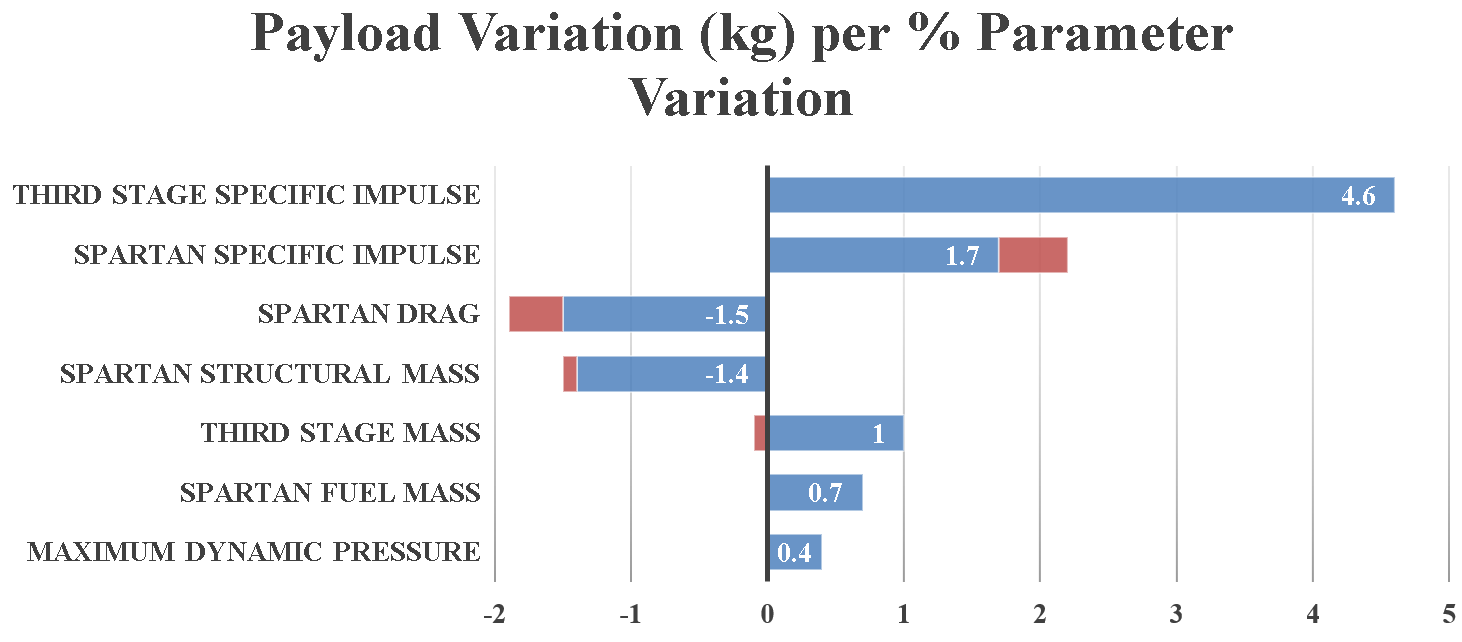
\includegraphics[width=0.8\linewidth]{figures/6_FlyBack/BarChart}
\caption{Sensitivity of design parameters. \textcolor{red}{include lines showing sensitivities without flyback}}
\label{fig:BarChart}
\end{figure}




\section{Sonic Boom Ground Effects}

The flight of a hypersonic vehicle has the potential to create significant overpressures on the ground due to sonic booms[CITEXX]. Even when the vehicle is flying at high altitudes, the overpressures on the ground may still be large enough to have detrimental effects on any populated areas being overflown. The overpressure from sonic booms can cause significant annoyance to the populace, or in more extreme cases, long term damage to building structures or peoples health. 
When the SPARTAN is launched to a sun synchronous orbit from the Equatorial Launch Australia launch site, it flies over a significant portion of Papua. Fortunately, Papua is sparsely populated, and the number of towns flown over by the SPARTAN will be low, however the effects on these population centres may still be significant. Although it is flying at high altitude, the SPARTAN is flying at hypersonic speeds, and creates significant sonic boom effects. In order to assess the impact of the SPARTAN's flight, the magnitude of the overpressure from its sonic booms must be calculated. 
\begin{figure}[ht]
	\centering
	\includegraphics[width=0.9\linewidth]{../LODESTAR_FINAL/Results/mode11/OverPressureStandard}
	\caption{}
	\label{fig:OverPressureStandard}
\end{figure}

The sonic boom overpressures are estimated using the 'first cut' estimation technique [CITEXX]. This estimation technique can approximate sonic boom overpressures moderately well, and is useful as a first approximation to the sonic boom overpressures generated by an aerospace vehicle. The overpressures generated by the SPARTAN are calculated over its trajectory, shown in Figure \ref{fig:OverPressureStandard}. It is found that overpressures of up to 375.3Pa occur during flight over land during the maximum payload-to-orbit trajectory of the SPARTAN. These overpressures have a low but significant probability of causing cosmetic damage to structures (~1.5\% for plaster and ~0.4\% for glass)[CITEXX-below]. In addition, overpressures of these magnitudes have been rated as unacceptably annoying to the majority populace being overflown, as shown in Figure \ref{fig:OverPressureResponse}. 
These overpressures indicate that overflight of populated areas may not be reasonable for the SPARTAN flying its maximum payload-to-orbit trajectory. 


%http://www.dtic.mil/dtic/tr/fulltext/u2/a028512.pdf





\section{Alternate Launch Locations}

A sun synchronous orbit may be attained in both northerly, and southerly directions. An alternate southerly launch is investigated for the rocket-scramjet-rocket launch system, in the case that flight over Papua is not possible. 


\begin{figure}[th]
\centering
\includegraphics[width=1\linewidth]{../LODESTAR_FINAL/Results/mode01/GroundTrackAlternate}
\caption{}
\label{fig:GroundTrackAlternate}
\end{figure}

\begin{table}
	\centering
\begin{tabular}{l c} 
	\hline \textbf{Trajectory Condition}
	& Alternate
	\\
	\hline \textbf{Payload to Orbit (kg)}
	& \PayloadToOrbitAlternate
	\\
	\textbf{Separation Alt, 1$\rightarrow$2 (km)}
	& \firstsecondSeparationAltAlternate
	\\
	\textbf{Separation v, 1$\rightarrow$2 (m/s)}
	& \firstsecondSeparationvAlternate
	\\
	\textbf{Separation $\gamma$, 1$\rightarrow$2 (m/s)}
	& \firstsecondSeparationgammaAlternate
	\\
	\textbf{Separation Alt, 2$\rightarrow$3 (km)}
	& \secondthirdSeparationAltAlternate
	\\
	\textbf{Separation $v$, 2$\rightarrow$3 (m/s)}
	& \secondthirdSeparationvAlternate
	\\
	\textbf{Separation $\gamma$, 2$\rightarrow$3 (deg)}
	& \secondthirdSeparationgammaAlternate
	\\
	\textbf{Separation $q$, 2$\rightarrow$3(kPa)}
	& \secondthirdSeparationqAlternate
	\\
	\textbf{2$^{nd}$ Stage L/D, 2$\rightarrow$3}
	& \secondthirdSeparationLDAlternate
	\\
	\textbf{2$^{nd}$ Stage Flight Time (s)}
	& \secondFlightTimeAlternate
	\\
	\textbf{3$^{rd}$ Stage $t$, $q >$ 5kpa (s)}
	& \thirdqOverFiveAlternate
	\\
	\textbf{3$^{rd}$ Stage max $\alpha$ (deg)}
	& \thirdmaxAoAAlternate
	\\
	\textbf{3$^{rd}$ Stage final v (m/s)}
	& \thirdcircvAlternate
	\\
	\textbf{3$^{rd}$ Stage final m (kg)}
	& \thirdcircmAlternate
	\\
	\hline 
\end{tabular} 
\end{table}

\section{Summary}
The fly-back trajectory of the SPARTAN hypersonic vehicle is investigated, from separation at 7.7$^\circ$S,145.0$^\circ$E to landing at 15.3$^\circ$S,144.9$^\circ$E, corresponding to a near 180$^\circ$ turn and a fly-back of 878km. The aerodynamics of the SPARTAN are calculated using CART3D, an inviscid CFD package, over the range of Mach numbers and angle of attack values of flight. The optimal trajectory of the SPARTAN is calculated, to fly-back to the initial launch position with minimum fuel. The optimal trajectory is calculated using the launch vehicle optimal control program LODESTAR. It is found that the SPARTAN is capable of returning to its initial launch position, using 166.0kg of fuel. The optimal trajectory terminates when SPARTAN reaches 200m altitude at a velocity of 119.8m/s. After this point, it is assumed that the SPARTAN lands on a traditional runway, at similar conditions to the space shuttle.  
This result indicates that the fly-back of a hypersonic launch vehicle from high velocity separation at a Mach number greater than nine, returning to its initial launch site using scramjet hypersonic airbreathing engines, is feasible. This fly-back to the the original launch site is a crucial component for low cost access-to-space using scramjets. 

The coefficient of drag of the SPARTAN and specific impulse of the scramjet engines were independently varied by $\pm10\%$ and the new optimal trajectories calculated to assess the robustness of the fly-back trajectory to uncertainties in vehicle aerodynamics and scramjet performance. It was found that a $\pm10\%$ variation in $C_D$ results in a +31.0\% or -34.9\% variation in fuel mass burned during fly-back, while a $\pm10\%$ variation in $I_{SP}$ results in a much smaller variation of -6.9\% or +13.8\%. These results indicate that the aerodynamics of a fly-back hypersonic accelerator are much more significant to the fly-back fuel usage than the performance of the scramjet engine. 

